\documentclass[titlepage,letterpaper,onecolumn,11pt,final]{report}

\usepackage{geometry}
\geometry{letterpaper,margin=1in,tmargin=0.5in}

\usepackage{graphicx}% Include figure files
\usepackage{dcolumn}% Align table columns on decimal point
\usepackage{bm}% bold math
\usepackage{amsmath}% bold math
\usepackage{mathtools} %boxes
%\usepackage{amssymb}
\usepackage{siunitx}% si units
\usepackage{color}
\usepackage{graphicx}
\usepackage{enumitem}
\usepackage{braket}
\usepackage{empheq} % boxes around multi line equations
\usepackage{csquotes}

\usepackage{hyperref}
\hypersetup{
    colorlinks,
    citecolor=black,
    filecolor=black,
    linkcolor=black,
    urlcolor=black
}

\usepackage{natbib}[numbers]
\usepackage{url}
\bibliographystyle{plainnat}

% User defined commands
\newcommand*\widefbox[1]{\fbox{\hspace{2em}#1\hspace{2em}}}

\newcommand{\Vx}{\hat{V}}
\newcommand{\Hx}{\hat{H}}
\newcommand{\Vsx}{\tilde{V} \left( x \right)}
\newcommand{\Pm}{\hat{p}}
\newcommand{\xp}{\hat{x}}
\newcommand{\Tv}{\hat{T}}
\newcommand{\ml}{m_{\ell}}
\newcommand{\ellv}{\hat{\vec{\ell}}}
\newcommand{\Sv}{\hat{\vec{s}}}
\newcommand{\che}{\chi_{e}}

\newcommand{\ahat}{\hat{a}}
\newcommand{\adag}{\hat{a}^{\dagger}}

\newcommand{\jup}{\hat{\jmath}_{^{_{_{+}}}}}
\newcommand{\jdown}{\hat{\jmath}_{^{_{_{-}}}}}
\newcommand{\jpm}{\hat{\jmath}_{^{_{_{\pm}}}}}

\newcommand{\jalpha}{\hat{\jmath}_{\alpha}}

\newcommand{\lx}{\hat{\ell}_{x}}
\newcommand{\ly}{\hat{\ell}_{y}}
\newcommand{\lz}{\hat{\ell}_{z}}
\newcommand{\ls}{\hat{\ell}^{2}}

\newcommand{\Sx}{\hat{s}_{x}}
\newcommand{\Sy}{\hat{s}_{y}}
\newcommand{\Sz}{\hat{s}_{z}}
\newcommand{\Ss}{\hat{s}^{2}}

\newcommand{\jx}{\hat{\jmath}_{x}}
\newcommand{\jy}{\hat{\jmath}_{y}}
\newcommand{\jz}{\hat{\jmath}_{z}}
\newcommand{\js}{\hat{\jmath}^{2}}

\newcommand{\ja}{\hat{\vec{\jmath}}_{1}}
\newcommand{\jxa}{\hat{\jmath}_{1 x}}
\newcommand{\jya}{\hat{\jmath}_{1 y}}
\newcommand{\jza}{\hat{\jmath}_{1 z}}
\newcommand{\jsa}{\hat{\jmath}_{1}^{2}}

\newcommand{\jb}{\hat{\vec{\jmath}}_{2}}
\newcommand{\jxb}{\hat{\jmath}_{2 x}}
\newcommand{\jyb}{\hat{\jmath}_{2 y}}
\newcommand{\jzb}{\hat{\jmath}_{2 z}}
\newcommand{\jsb}{\hat{\jmath}_{2}^{2}}

\newcommand{\jv}{\hat{\vec{\jmath}}}

\newcommand{\comm}[2]{[ #1 , #2 ]}
\newcommand{\Ham}{\hat{\mathcal{H}}}
\newcommand{\Hamh}{\hat{\mathcal{H}}_{H}}
\newcommand{\Hamho}{\hat{\mathcal{H}}_{HO}}
\newcommand{\Hamo}{\hat{\mathcal{H}}_{0}}

\newcommand{\partder}[2]{\frac{\partial #1}{\partial #2}}
\newcommand{\partsqr}[2]{\frac{\partial^{2} #1}{\partial #2^{2}}}

\newcommand{\partderb}[2]{\frac{\partial}{\partial #2} #1}
\newcommand{\partsqrb}[2]{\frac{\partial^{2}}{\partial #2^{2}} #1}

\newcommand{\psx}{\Psi (x)}
\newcommand{\psxt}{\Psi (\mathbf{x},t)}
\newcommand{\psxs}{\Psi^{*} (\mathbf{x},t)}

\newcommand{\psl}{\Psi (L)}
\newcommand{\pso}{\Psi (0)}
\newcommand{\dpsx}{\frac{d \Psi (x)}{d x}}
\newcommand{\dpsl}{\frac{d \Psi (L)}{d x}}
\newcommand{\dpso}{\frac{d \Psi (0)}{d x}}

\newcommand{\ketb}[1]{\ket{\mathbf{#1}}}
\newcommand{\brab}[1]{\bra{\mathbf{#1}}}

\newcommand{\gama}{\gamma^{0}}
\newcommand{\gamb}{\gamma^{1}}
\newcommand{\gamc}{\gamma^{2}}
\newcommand{\gamd}{\gamma^{3}}
\newcommand{\game}{\gamma^{4}}
\newcommand{\gamf}{\gamma^{5}}

\DeclareMathOperator{\Tr}{Tr}

\numberwithin{equation}{section}
\numberwithin{figure}{section}

\begin{document}

\hypersetup{pageanchor=false}
\begin{titlepage}
	\centering
	\includegraphics[width=0.15\textwidth]{UBC_logo.png}\par
	\vspace{1cm}
	{\scshape\LARGE University of British Columbia \par}
	\vspace{1cm}
	{\scshape\Large CHEM 501: Project\par}
	\vspace{1.5cm}
	{\huge\bfseries Relativistic Quantum Mechanics\par}
	\vspace{2cm}
	{\Large\itshape Hayden Scheiber\par}
	\vfill
	supervised by\par
	Dr.~Mark \textsc{Thachuk}

	\vfill

% Bottom of the page
	{\large \today\par}
\end{titlepage}

\hypersetup{pageanchor=true}

\tableofcontents

\chapter{Background}

The goal of relativistic quantum mechanics is to construct wavefunctions, operators, and their eigenvalues that are consistent with special (and ultimately general) relativity. Such a theory should be in agreement with the postulates of quantum mechanics. In these notes I will attempt to explore relativistic quantum mechanics---following chapter eight of~\cite{b:ModernQM}---with the ultimate goal of deriving the electron spin from first principles.

In order to begin talking about relativistic quantum mechanics, we first need to explore special relativity. Specifically, we need to know what a relativistic version of quantum mechanics must incorporate in order to be in agreement with special relativity.

\section{Special Relativity}

Under classical Galilean physics, space is a totally separate entity from time. The geometry of the three spatial coordinates are decoupled from the geometry of the single time coordinate. This implies that both time intervals and distances are absolute. In fact, the \emph{Galilean principle of relativity} asserts that \emph{all} of the laws of mechanics are the same in all inertial frames of reference. This is equivalent to stating that transformations of inertial reference frame leave the laws of physics invariant. 

Galilean physics---and indeed our everyday intuition about the universe---claims that two observers traveling at different speeds will always agree on the the ordering of events and the spatial distance between points. They will not, however, agree on the velocity of objects (including massless particles). It makes sense to say ``all of space at a certain time''. Mathematically, transforming a point between one inertial frame ($t,\ x,\ y,\ z$) and another ($t',\ x',\ y',\ z'$) moving at velocity $\mathbf{v}$ relative to the first is done by the Galilean transformation equations
\begin{subequations}
\begin{align}
	\label{eq:Galilean_transform}
	t' &= t \\
	\mathbf{r}'(t) &= \mathbf{r}(t) - \mathbf{v}t .
\end{align}
\end{subequations}

Where $\mathbf{r}$ is the position vector ($x,\ y,\ z$) at time $t$. Notice that under this paradigm, the speed that light travels at will depend on the frame of reference. For example, if a photon is moving at $c$ relative to some frame of reference $(t,\ x,\ y,\ z)$, then it will appear as a static electric and magnetic field in a frame moving at $\mathbf{v} = c$ in the same direction. This particular thought-experiment lead Einstein to his famous \emph{principle of special relativity}, because Maxwell's equations predict that a static electric or magnetic field can exist only near a charged object or a steady current, not in empty space. Figure~\ref{fig:galilean} provides another example where the second reference frame is moving at 0.5c.

In fact, the wave solution to Maxwell's equations predicts that the speed of light waves should always be a particular constant $c$. Scientists before Einstein reasoned that there must be some preferred reference frame that contained the ``luminiferous ether'', with was the supposed medium through which light traveled with velocity $c$. If that were the case, only in the particular reference frame of the luminiferous ether would Maxwell's equations hold true, which seems to contradict the Galilean principle of relativity.

\begin{figure}[!htb]
	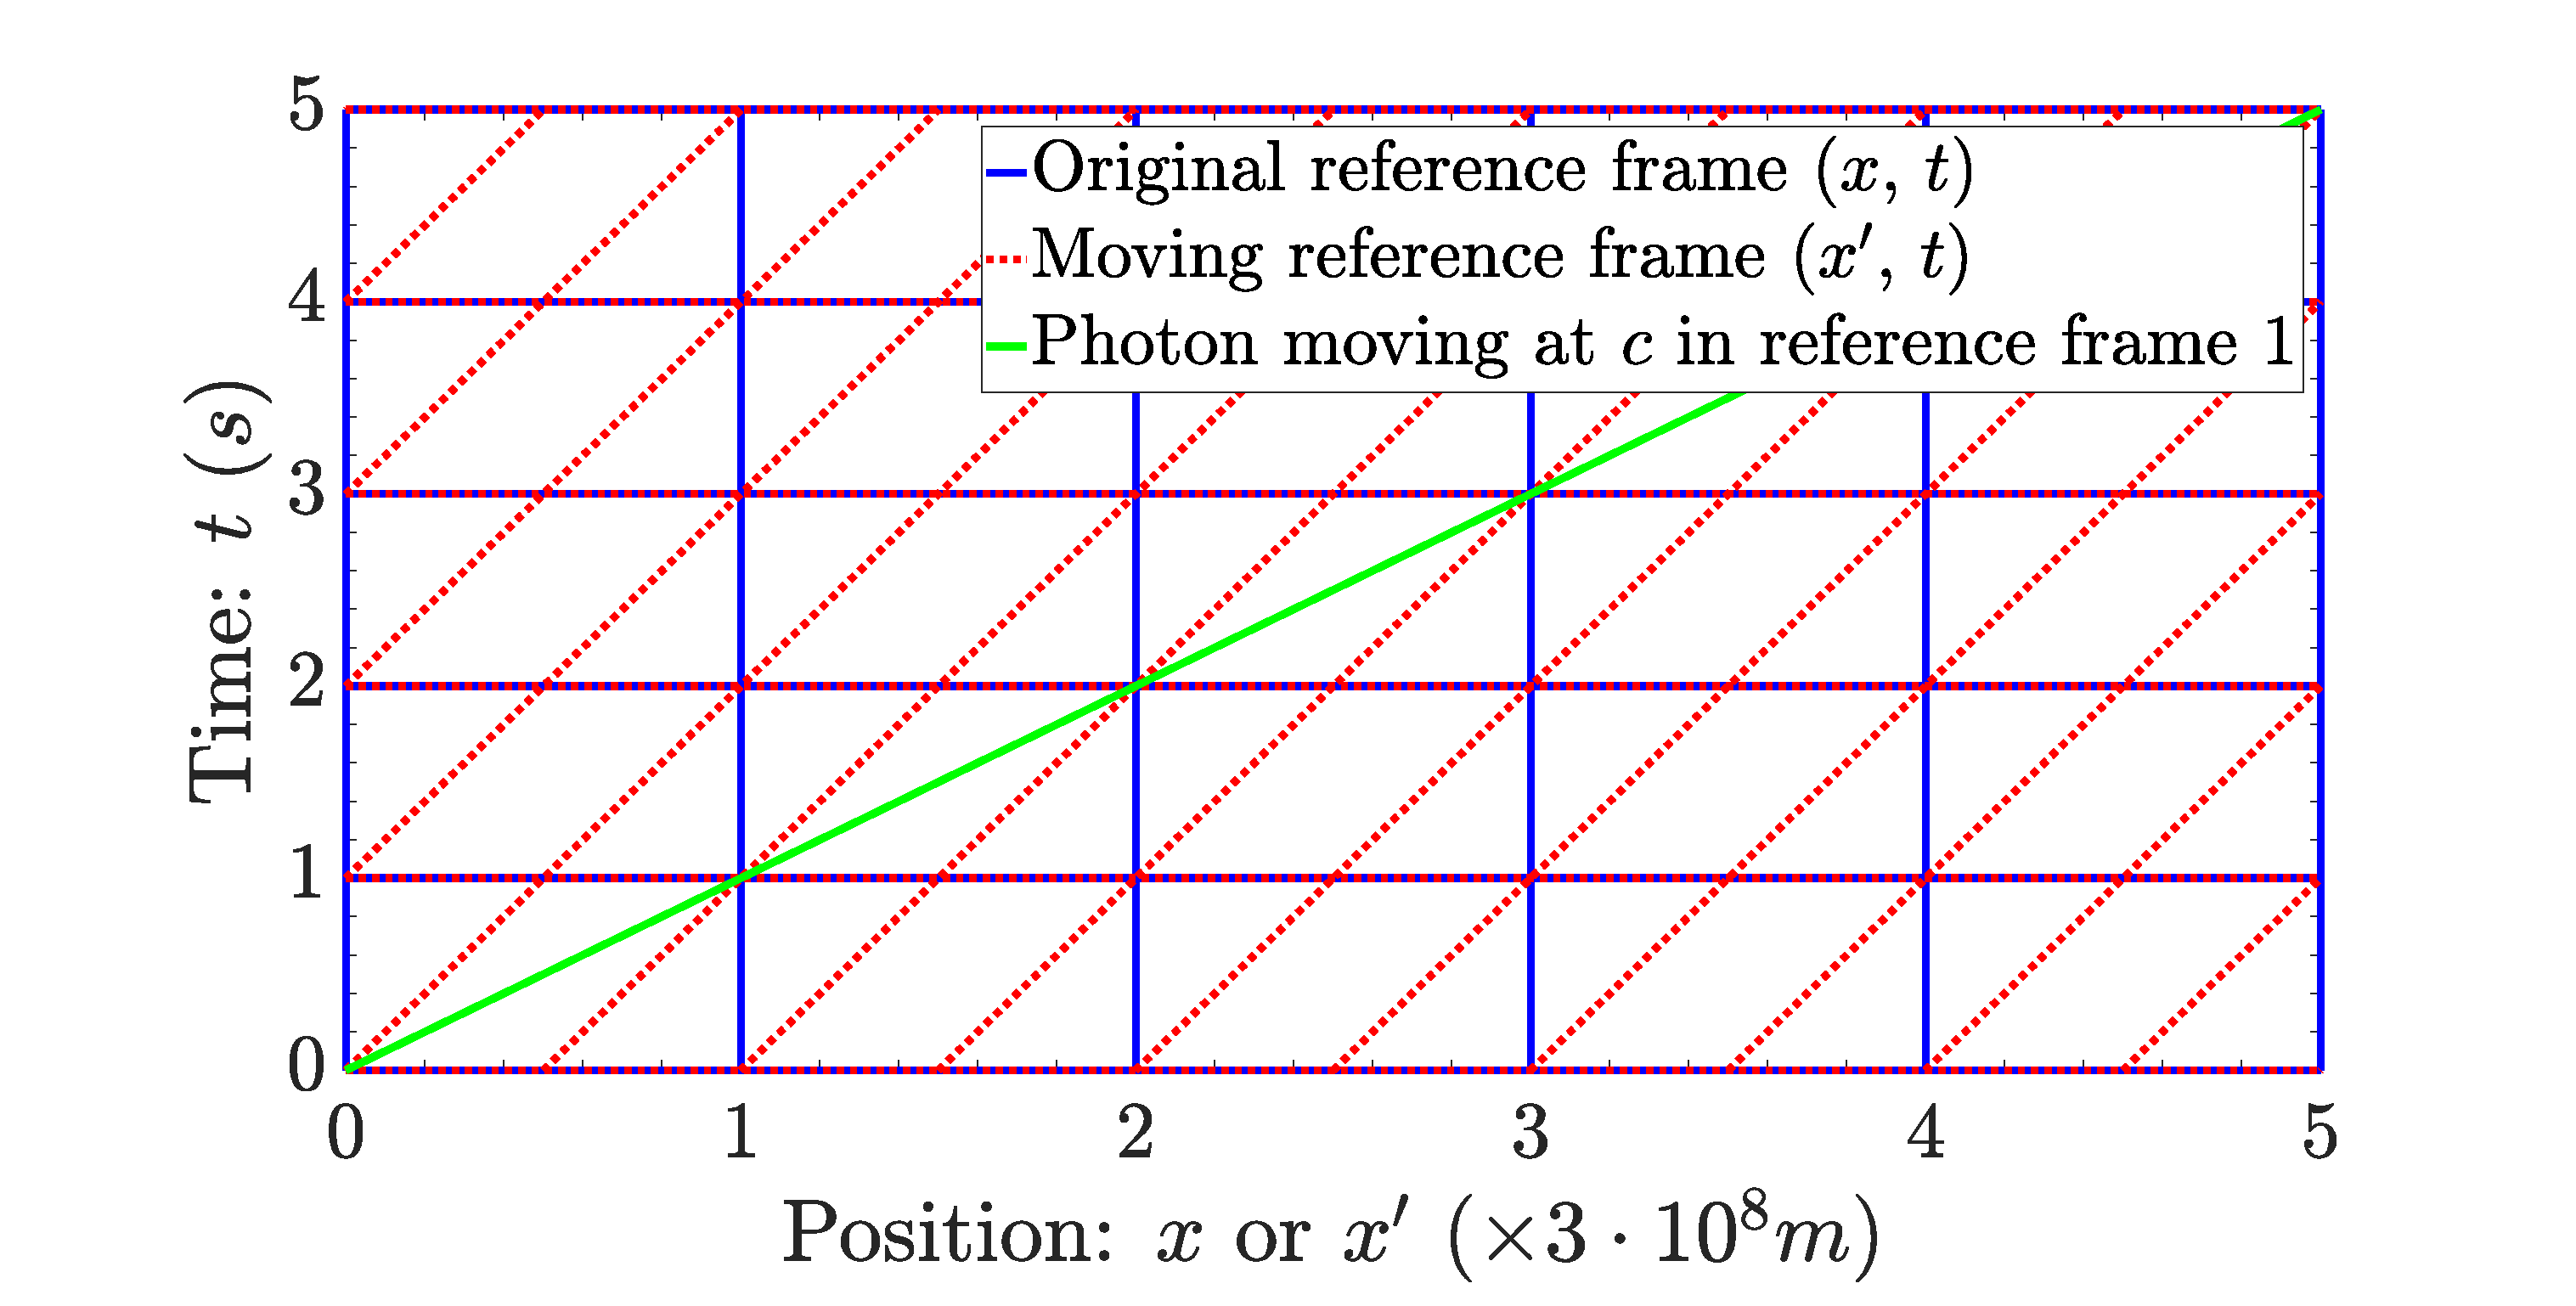
\includegraphics[trim={3.3cm 0.1cm 4.5cm 1cm},clip,width=\textwidth]{galilean.eps}
	\caption{\label{fig:galilean} Visualization of a Galilean Transform in one spatial dimension $x$ and one time dimension $t$. Moving along a vertical blue path traces out the trajectory of a stationary point traveling through time in the first reference frame. The green line traces out the path of a photon that starts at point ($t=0$, $x=0$) and heads in the positive $x$ direction. From the point of view of another observer traveling at $0.5c$ (red lines), the speed of the photon appears to be $0.5c$. To see this, notice that after 1 second, the green path is only $0.5 s \times c$ ahead of the location of the red path that starts at ($t=0$, $x=0$). After 2 seconds, the photon is $1 s \times c$ ahead of the moving observer.}
\end{figure}

Of course, experiment has since proven beyond a doubt that the speed of light is the same in \emph{any} inertial frame of reference! In order to make sense of this, we will embrace Einstein's principle of special relativity. This will force us to challenge the assumption that time and space are both separately invariant to changes in inertial frame of reference. The principle of special relativity states that all laws of physics, and the physical constants contained within them (such as the speed of light), are the same for \emph{any} inertial frame of reference. Einstein's task was then to find a geometry of space and time that would support such a principle, which lead him to develop his theory of special relativity.

\section{The Spacetime Interval}

In special relativity, time and space coordinates become interwoven into a single coordinate system called spacetime. Under this new paradigm, the time and distance between events become combined into a single \emph{spacetime interval}, which describes the spacetime ``distance'' between two events
\begin{gather}
	\label{eq:spacetime_interval}
	\Delta s^{2} = (c \Delta t)^{2} - (\Delta x)^{2} - (\Delta y)^{2} - (\Delta z)^{2} .
\end{gather}

Note that some authors define the spacetime interval with the opposite sign for time and space components; this does not effect the end results. The spacetime interval is the 4D special relativity analogue of the squared distance between two points in 3D space (note $\Delta s^{2}$ is usually defined as the spacetime interval, not $\Delta s$). In special relativity the spacetime interval is invariant, independent of the observer's inertial frame of reference. In order to allow this, neither the time nor the space between events can be separately invariant between different inertial frames of reference. This is very different from our everyday understanding of the universe, but has nevertheless been proven true. 

One can observe that the spacetime interval has a similar form to the Pythagorean formula, where the sign of the time component is opposite that of the spatial components. Why is it so? The spacetime interval follows directly from the construction of a geometry of spacetime that is constrained by the principle of special relativity. It also appears to confirm our intuition that time is not simply another spatial dimension; it is somehow \emph{different} than the other three dimensions.

Because it contains both negative and positive terms, the spacetime interval $\Delta s^{2}$ can be either positive, zero, or negative. For example, in the case where an object has not changed it's spatial position (with respect to a particular reference frame) but time has passed, the spacetime interval will be positive. Positive spacetime intervals are known as ``time-like'' trajectories. Massive objects always travel through spacetime along time-like trajectories. When the spacetime interval is negative, physicists call this a ``space-like'' path. Space-like paths are separated by more space than is possible to traverse while moving at the speed of light for the given time. Events separated by a space-like path cannot be causally linked. That is, two events separated by a space-like trajectory cannot have information travel between them. When the spacetime interval is exactly zero, $(c \Delta t)^{2} = (\Delta x)^{2} + (\Delta y)^{2} + (\Delta z)^{2}$. The change in spatial distance is exactly equal to the distance covered by an object moving at $c$ for a time $\Delta t$. Such paths correspond to the paths taken through spacetime by all massless particles, such as photons. Hence, they are called ``light-like'' paths.

What kinds of transformations will leave the spacetime interval $\Delta s^{2}$ unchanged? To answer this question, we must first introduce some essential ideas in vector calculus that will help us tremendously when discussing special relativity and later when discussing relativistic quantum mechanics.

\section{Vector Calculus for Special Relativity}

To represent vectors of four coordinates in spacetime---henceforth termed \emph{four-vectors}---for a particular reference frame, physicists use Greek superscripts (or subscripts, explained later) such as
\begin{gather}
	\label{eq:contravariant_4v}
	x^{\mu} \equiv
	\begin{bmatrix}
		x^{0} \\[6pt]
		x^{1} \\[6pt]
		x^{2} \\[6pt]
		x^{3} 
	\end{bmatrix}
	=
	\begin{bmatrix}
		c t \\[6pt]
		x \\[6pt]
		y \\[6pt]
		z
	\end{bmatrix}
	.
\end{gather}
%
To represent three-vectors (such as a point in 3D space) Latin superscripts are used, as in
\begin{gather}
	x^{i} \equiv
	\begin{bmatrix}
		x^{1} \\[6pt]
		x^{2} \\[6pt]
		x^{3}
	\end{bmatrix}
	=
	\begin{bmatrix}
		x \\[6pt]
		y \\[6pt]
		z
	\end{bmatrix}
	.
\end{gather}

By convention, if an index is repeated in expressions that use this notation, summation across that index is implied. This is often called \emph{contraction}; it always occurs between subscripted and superscripted indices. For example, 
\begin{gather}
	x^{\mu}y_{\mu} = \sum_{\mu = 0}^{3}{x^{\mu}y_{\mu}} = x^{0}y_{0} + x^{1}y_{1} + x^{2}y_{2} + x^{3}y_{3}.
\end{gather}

The \emph{spacetime metric} $\eta$ is a collection of 16 numbers, which can be arranged into a $4 \times 4 $ tensor matrix. The spacetime metric contains all information about the geometric and causal structure of the spacetime it describes. It appears very often in relativity, and is in many ways comparable to the $3 \times 3$ identity matrix in Galilean relativity. In special relativity, we only deal with flat spacetime, so the spacetime metric has the very simple form
\begin{gather}
	\eta_{\mu \nu} \equiv
	\begin{bmatrix}
		\eta_{0 0} & \eta_{0 1}  & \eta_{0 2}  & \eta_{0 3} \\
		\eta_{1 0} & \eta_{1 1}  & \eta_{1 2}  & \eta_{1 3} \\
		\eta_{2 0} & \eta_{2 1}  & \eta_{2 2}  & \eta_{2 3} \\
		\eta_{3 0} & \eta_{3 1}  & \eta_{3 2}  & \eta_{3 3} \\
	\end{bmatrix}
	=
	\begin{bmatrix}
		1 & 0  & 0  & 0 \\
		0 & -1 & 0  & 0 \\
		0 & 0  & -1 & 0 \\
		0 & 0  & 0  & -1 \\
	\end{bmatrix}
	.
\end{gather}
%
The spacetime interval in this new notation is simply
\begin{equation}
\begin{split}
	\label{eq:spacetime_condensed}
	\Delta s^{2} &= (\Delta x^{\mu}) \eta_{\mu \nu} (\Delta x^{\nu}) \\
	&= (\Delta x^{\mu}) \left( \eta_{\mu 0} \Delta x^{0} + \eta_{\mu 1} \Delta x^{1} + \eta_{\mu 2} \Delta x^{2} + \eta_{\mu 3} \Delta x^{3} \right) \\
	&= (\Delta x^{\mu}) \left( \Delta x_{\mu} \right) \\
	&= (c \Delta t)^{2} - (\Delta x)^{2} - (\Delta y)^{2} - (\Delta z)^{2}.
\end{split}
\end{equation}
%
Here we have introduced the difference between the superscript and subscript forms of the four-vector. A four-vector written with a superscript is known as a ``contravariant'' four-vector. A subscripted four-vector is known as a ``covariant'' four-vector. For any set of four coordinates, the covariant four-vector is simply $x_{\mu} = \eta_{\mu \nu} x^{\nu}$. Note that we can also write the contravariant four-vector in terms of the covariant one with $x^{\mu} = \eta^{\mu \nu} x_{\nu}$. $\eta^{\mu \nu}$ is the inverse metric tensor, which has the property $\eta_{\nu \alpha} \eta^{\alpha \mu} = \delta^{\mu}_{\nu}$, where $\delta^{\mu}_{\nu}$ is the Kronecker delta. It is easy to show that the components of the inverse metric tensor are exactly the same as the metric tensor. In the context of special and general relativity, the inner product between contravariant and covariant four-vectors is defined as the \emph{dot product}, and is automatically invariant to changes in inertial reference frame due to the implicit inclusion of the spacetime metric.

Now imagine we wish to transform a point in spacetime represented by the four-vector $x^{\nu}$ into a different reference frame. We can do this using some $4 \times 4$ transformation matrix ${a^{\mu}}_{\nu}$. The transformation equation is simply
\begin{align}
	\label{eq:arb_transform}
	{x'}^{\mu} = {a^{\mu}}_{\nu} x^{\nu} .
\end{align}
%
We want to ensure that the transformation ${a^{\mu}}_{\nu}$ leaves the spacetime interval unchanged. This means that
\begin{equation}
\begin{split}
	\label{eq:transform_intermediate}
	{x'}^{\alpha} {x'}_{\alpha} &= x^{\mu} x_{\mu} \\
	\eta_{\alpha \beta} {x'}^{\alpha} {x'}^{\beta} &= \eta_{\mu \nu} x^{\mu} x^{\nu} .
\end{split}
\end{equation}
%
This is a good moment to pause and note that---strictly speaking---when using the summation convention, we need not think of the four-vectors as matrices that cannot commute. They are simply a grouping of components, and the matching indices automatically take care of any contraction, allowing commutation. With that in mind, we can substitute equation~\ref{eq:arb_transform} into equation~\ref{eq:transform_intermediate} to get
\begin{equation}
\begin{split}
	\eta_{\alpha \beta} {a^{\alpha}}_{\mu} x^{\mu} {a^{\beta}}_{\nu} x^{\nu} &= \eta_{\mu \nu} x^{\mu} x^{\nu} \\
	x^{\mu} x^{\nu} \left( {a^{\alpha}}_{\mu} \eta_{\alpha \beta} {a^{\beta}}_{\nu} - \eta_{\mu \nu} \right) &= 0 .
\end{split}
\end{equation}
This means that any transformation ${a^{\alpha}}_{\mu}$ to a new inertial frame of reference must obey
\begin{gather}
	\label{eq:Lorentz_transforms}
	{a^{\alpha}}_{\mu} \eta_{\alpha \beta} {a^{\beta}}_{\nu} = \eta_{\mu \nu} .
\end{gather}

The set of all possible transformations that obey equation~\ref{eq:Lorentz_transforms} are called the Lorentz transformations. The set of Lorentz transformations that leave the time component of a four-vector unchanged are simply the spatial rotations. The class of Lorentz transforms that change the time component are called Lorentz boosts, and always correspond to a change in reference frame differing by a constant velocity. There are six basis Lorentz transforms from which all other possible Lorentz transforms can be constructed by linear combination. They are the three orthogonal spatial rotations and the three boosts that ``mix'' time and a single spatial component.

Up until this point, we have not seen a definition for covariant and contravariant four-vectors. The true definition of a contravariant vector is one that transforms under any Lorentz transformation as
\begin{gather}
	\label{def:contravariant}
	{x'}^{\mu} = {a^{\mu}}_{\nu} x^{\nu}.
\end{gather}
%
How do covariant vectors transform under the Lorentz transformations? We can use the fact that in general, $x_{\mu} = \eta_{\mu \nu} x^{\nu}$ and $x^{\mu} = \eta^{\mu \nu} x_{\nu}$ to write
\begin{gather}
	{x'}_{\mu} = \eta_{\mu \nu} {x'}^{\nu} = \eta_{\mu \nu} {a^{\nu}}_{\alpha} x^{\alpha} = \eta_{\mu \nu} {a^{\nu}}_{\alpha} \eta^{\alpha \beta} x_{\beta} .
\end{gather}
%
We then define
\begin{gather}
	\label{eq:covariant_transform}
	{a_{\mu}}^{\beta} \equiv \eta_{\mu \nu} {a^{\nu}}_{\alpha} \eta^{\alpha \beta}
\end{gather}
so that
\begin{gather}
	\label{def:covariant}
	{x'}_{\mu} = {a_{\mu}}^{\beta} x_{\beta} .
\end{gather}
The formal definition of a covariant four-vector is one that transforms according to equation~\ref{def:covariant}. 

It is interesting to note that for any general Lorentz transform, ${a^{\alpha}}_{\nu}$ and ${a_{\alpha}}^{\mu}$ are always inverses. This means that 
\begin{gather}
	{a^{\alpha}}_{\nu} {a_{\alpha}}^{\mu} = \delta^{\mu}_{\nu} .
\end{gather}
%
We can easily prove this by multiplying equation~\ref{eq:Lorentz_transforms} by $\eta^{\nu \sigma}$, giving us
\begin{subequations}
\begin{align}
	\label{eq:lorentz_inversions1}
	{a^{\alpha}}_{\mu} \eta_{\alpha \beta} {a^{\beta}}_{\nu} \eta^{\nu \sigma} &= \eta_{\mu \nu} \eta^{\nu \sigma} \\
	\label{eq:lorentz_inversions2}
	{a^{\alpha}}_{\mu} {a_{\alpha}}^{\sigma} &= \delta^{\sigma}_{\mu},
\end{align}
\end{subequations}
where the last line follows from the definition given in equation~\ref{eq:covariant_transform}, and the fact that $\eta_{\mu \nu} \eta^{\nu \sigma} = \delta^{\sigma}_{\mu}$.

The information given thus far is rather abstract, and it is definitely worth going through an example that demonstrates the mathematics of this section. The following $4 \times 4$ matrix can be used to represent a Lorentz boost ${a^{\mu}}_{\nu}$ in the x-direction:
\begin{gather}
{a^{\mu}}_{\nu} =
	\begin{bmatrix}
	 \frac{1}{\sqrt{1-\frac{V^2}{c^2}}} & -\frac{\frac{V}{c}}{\sqrt{1-\frac{V^2}{c^2}}} & 0 & 0 \\[10pt]
	 -\frac{\frac{V}{c}}{\sqrt{1-\frac{V^2}{c^2}}} & \frac{1}{\sqrt{1-\frac{V^2}{c^2}}} & 0 & 0 \\[10pt]
	 0 & 0 & 1 & 0 \\[10pt]
	 0 & 0 & 0 & 1
	\end{bmatrix}  .
\end{gather}
%
We can use equation~\ref{def:contravariant} to apply this transformation to the matrix representation of some arbitrary contravariant four-vector
\begin{gather}
	{x'}^{\mu} = 
	\begin{bmatrix}
	 ct' \\[13pt]
	 x' \\[13pt]
	 y' \\[13pt]
	 z' 
	\end{bmatrix}
	=
	{a^{\mu}}_{\nu} x^{\nu} =
	\begin{bmatrix}
	 ct \\[13pt]
	 x \\[13pt]
	 y \\[13pt]
	 z 
	\end{bmatrix}
	\begin{bmatrix}
	 \frac{1}{\sqrt{1-\frac{V^2}{c^2}}} & -\frac{\frac{V}{c}}{\sqrt{1-\frac{V^2}{c^2}}} & 0 & 0 \\[10pt]
	 -\frac{\frac{V}{c}}{\sqrt{1-\frac{V^2}{c^2}}} & \frac{1}{\sqrt{1-\frac{V^2}{c^2}}} & 0 & 0 \\[10pt]
	 0 & 0 & 1 & 0 \\[10pt]
	 0 & 0 & 0 & 1
	\end{bmatrix} .
\end{gather}
%
This leads to the following set of transformation equations describing the transformed contravariant vector:
\begin{subequations}
\begin{align}
 {x'}^{0} &= ct'= \frac{ct - \frac{V}{c}x}{\sqrt{1-\frac{V^2}{c^2}}}, \\
 {x'}^{1} &= x' = \frac{x - \frac{V}{c}ct}{\sqrt{1-\frac{V^2}{c^2}}}, \\
 {x'}^{2} &= y' = y, \\
 {x'}^{3} &= z' = z.
\end{align}
\end{subequations}
%
How does ${a_{\mu}}^{\beta}$ look in matrix form? It is easy to calculate using equation~\ref{eq:covariant_transform}. Adopting the same example transformation matrix ${a^{\nu}}_{\alpha}$, it is just
\begin{subequations}
\begin{align}
	{a_{\mu}}^{\beta} &= \eta_{\mu \nu} {a^{\nu}}_{\alpha} \eta^{\alpha \beta} \\
	&=
	\begin{bmatrix}
	 1 & 0 & 0 & 0 \\[13pt]
	 0 & -1 & 0 & 0 \\[13pt]
	 0 & 0 & -1 & 0 \\[13pt]
	 0 & 0 & 0 & -1
	\end{bmatrix}
	\begin{bmatrix}
	 \frac{1}{\sqrt{1-\frac{V^2}{c^2}}} & -\frac{\frac{V}{c}}{\sqrt{1-\frac{V^2}{c^2}}} & 0 & 0 \\[10pt]
	 -\frac{\frac{V}{c}}{\sqrt{1-\frac{V^2}{c^2}}} & \frac{1}{\sqrt{1-\frac{V^2}{c^2}}} & 0 & 0 \\[10pt]
	 0 & 0 & 1 & 0 \\[10pt]
	 0 & 0 & 0 & 1
	\end{bmatrix}
	\begin{bmatrix}
	 1 & 0 & 0 & 0 \\[13pt]
	 0 & -1 & 0 & 0 \\[13pt]
	 0 & 0 & -1 & 0 \\[13pt]
	 0 & 0 & 0 & -1
	\end{bmatrix} \\
	&=
	\begin{bmatrix}
	 \frac{1}{\sqrt{1-\frac{V^2}{c^2}}} & \frac{\frac{V}{c}}{\sqrt{1-\frac{V^2}{c^2}}} & 0 & 0 \\[10pt]
	 \frac{\frac{V}{c}}{\sqrt{1-\frac{V^2}{c^2}}} & \frac{1}{\sqrt{1-\frac{V^2}{c^2}}} & 0 & 0 \\[10pt]
	 0 & 0 & 1 & 0 \\[10pt]
	 0 & 0 & 0 & 1
	\end{bmatrix}.
\end{align}
\end{subequations}
%
Applying this to a covariant four-vector, constructed from $x_{\mu} = \eta_{\mu \nu} x^{\nu}$ we get
\begin{gather}
	{x'}_{\mu} =
	\begin{bmatrix}
	 ct \\[13pt]
	 -x \\[13pt]
	 -y \\[13pt]
	 -z 
	\end{bmatrix}
	\begin{bmatrix}
	 \frac{1}{\sqrt{1-\frac{V^2}{c^2}}} & \frac{\frac{V}{c}}{\sqrt{1-\frac{V^2}{c^2}}} & 0 & 0 \\[10pt]
	 \frac{\frac{V}{c}}{\sqrt{1-\frac{V^2}{c^2}}} & \frac{1}{\sqrt{1-\frac{V^2}{c^2}}} & 0 & 0 \\[10pt]
	 0 & 0 & 1 & 0 \\[10pt]
	 0 & 0 & 0 & 1
	\end{bmatrix} ,
\end{gather}
%
which leads to a set of equations that describes the components of the transformed covariant four-vector:
\begin{subequations}
\begin{align}
 {x'}_{0} &= ct'= \frac{ct - \frac{V}{c}x}{\sqrt{1-\frac{V^2}{c^2}}}, \\
 {x'}_{1} &= -x' = -\frac{x - \frac{V}{c}ct}{\sqrt{1-\frac{V^2}{c^2}}}, \\
 {x'}_{2} &= -y' = -y, \\
 {x'}_{3} &= -z' = -z.
\end{align}
\end{subequations}
As expected, the components are identical to $\eta_{\mu \nu} {x'}^{\nu}$.

There is actually one other rather trivial class of transformation that leaves the spacetime interval invariant, and it is not considered a Lorentz transformation. It is the so-called spacetime translation. If $\Delta x^{\mu} \equiv x^{\mu} - x^{\mu'}$, then it is clear that adding a constant to any of the components of both $x^{\mu}$ \emph{and} $x^{\mu'}$ will leave $\Delta x^{\mu}$ unchanged, and hence $(\Delta x^{\mu})^{2}$ unchanged. As discussed, the transformation matrices that solve equation~\ref{eq:Lorentz_transforms} are known as Lorentz transformations. The set of all possible Lorentz transformation matrices ${a^{\mu}}_{\nu}$ is called the Lorentz group. The Lorentz group combined with the spacetime translation is known as the Poincar\'{e} group. 

To give the reader another concrete example a of Lorentz transformation, below is the matrix representation of rotation about the z-axis by an angle $\theta$. This transform looks like
\begin{gather}
	\label{eq:Lorentz_rotation}
	{a^{\mu}}_{\nu} =
	\begin{bmatrix}
		1  & 0             & 0             & 0 \\
		0  & \cos \theta & \sin \theta & 0 \\
		0  &-\sin \theta & \cos \theta & 0 \\
		0  & 0             & 0             & 1 \\
	\end{bmatrix}
	.
\end{gather}

Hopefully, the reader can convince themselves that ${a^{\alpha}}_{\mu} \eta_{\alpha \beta} {a^{\beta}}_{\nu} = \eta_{\mu \nu}$ in this case (note that in matrix notation ${a^{\beta}}_{\nu}$, is the transpose of ${a^{\alpha}}_{\mu}$). The Lorentz boost can also be written in a form remarkably similar to a rotation between a spatial dimension and time, where the sines and cosines are replaced by their hyperbolic versions and a sign is changed. For example, a Lorentz boost in the x-direction can be written
\begin{gather}
	\label{eq:Lorentz_boost}
	{a^{\alpha}}_{\mu} =
	\begin{bmatrix}
		\cosh \phi  & -\sinh \phi & 0 & 0 \\
		-\sinh \phi & \cosh \phi  & 0 & 0 \\
		0  						& 0             & 1 & 0 \\
		0  						& 0             & 0 & 1 \\
	\end{bmatrix}
	,
\end{gather}
%
where $\phi$ is a parameter in the range $(-\infty, \infty)$. As discussed, Lorentz boosts correspond to changing coordinates into a frame of reference which is traveling at a constant velocity with respect to the initial reference frame. We can interpret the transform matrix as follows: each column of ${a^{\alpha}}_{\mu}$ corresponds to a transformed coordinate $x'^{\mu}$ in the basis of the old coordinates $x^{\mu}$. The transformed coordinates of the above example are
\begin{subequations}
\begin{align}
	\label{eq:Lorentz_boost_t}
	t' &= t \cosh \phi - x \sinh \phi ,\\
	\label{eq:Lorentz_boost_x}
	x' &= -t \sinh \phi + x \cosh \phi ,\\
	\label{eq:Lorentz_boost_y}
	y' &= y ,\\
	\label{eq:Lorentz_boost_z}
	z' &= z .
\end{align}
\end{subequations}

Let's track the movement of the origin of the new reference frame $x' = 0$ from the point of view of the old reference frame. This amounts to
\begin{equation}
\begin{split}
	x' = 0  &= -t \sinh \phi + x \cosh \phi \\
	t \sinh \phi &= x \cosh \phi \\
	v = \frac{x}{t} &= \frac{\sinh \phi}{\cosh \phi } = \tanh \phi .
\end{split}
\end{equation}
%
So the velocity of the transformed reference frame from the point of view of the old reference frame is $v = \tanh \phi$. Inverting this, we can write $\phi = \tanh^{-1} \left( v \right)$. Plugging this result back in to equations~\ref{eq:Lorentz_boost_t} and~\ref{eq:Lorentz_boost_x} yields
\begin{subequations}
\begin{align}
	t' &= t \cosh \left( \tanh^{-1} \left( v \right) \right) - x \sinh \left( \tanh^{-1} \left( v \right) \right) \\
	x' &= -t \sinh \left( \tanh^{-1} \left( v \right) \right) + x \cosh \left( \tanh^{-1} \left( v \right) \right) .
\end{align}
\end{subequations}
%
These equations can be simplified with a bit of algebra---after plugging in the definitions of the hyperbolic sine and cosine functions---to 
\begin{subequations}
\begin{align}
	t' &= \frac{t - x v}{\sqrt{1 - v^{2}}} \\
	x' &= \frac{x - v t}{\sqrt{1 - v^{2}}} .
\end{align}
\end{subequations}
%
If we write the velocity $v$ as a fraction of the speed of light $\frac{v}{c}$ and note that $t$ and $t'$ are really the distances $c t$ and $c t'$, we recover the common form of the Lorentz boost equations:
\begin{subequations}
\begin{align}
	t' &= \frac{t - \frac{v}{c^{2}}x}{\sqrt{1 - \frac{v^{2}}{c^{2}}}} ,\\
	x' &= \frac{x - vt}{\sqrt{1 - \frac{v^{2}}{c^{2}}}} ,\\
	y' &= y ,\\
	z' &= z .
\end{align}
\end{subequations}
%
The Lorentz boosts are the only transformations into another inertial reference frame with different velocity that ensure the speed of light $c$ and all other physical constants are unchanged.

\begin{figure}[!htb]
\centering
\includegraphics[trim={0cm 0cm 0cm 0cm},clip,width=0.5\textwidth]{lorentz_Transformation.jpg}
\caption{\label{fig:lorentz} Visualization of a Lorentz boost in the $x$-direction. The green line represents a photon of light moving in the $x$-direction in both frames of reference. Notice that, unlike the Galilean transformations, the time is allowed to stretch as a result of Lorentz transformations. Faster velocities result in a stretched time axis from the point of view of the initial reference frame. This is known as time dilation. This transformation allows light to remain at speed $c$ in both frames of reference.}
\end{figure}

We can easily show that this transformation does indeed conserve the speed of light $c$ by imagining a photon in the first reference frame, moving at $c$ along the x direction. We shall ignore the y and z coordinates for the sake of simplicity. After some time $t = \tau$, the photon will have traveled a distance $x = c\tau$. Its speed in this frame is $\frac{x}{t} = \frac{c\tau}{\tau} = c$. If we observe the photon from another inertial frame of reference moving at velocity $v$ with respect to the first, then the light will have traveled a distance
\begin{gather}
	x' = \frac{c\tau - v\tau}{\sqrt{1 - \frac{v^{2}}{c^{2}}}} = c \tau \Bigg( \frac{1 - \frac{v}{c}}{\sqrt{1 - \frac{v^{2}}{c^{2}}}} \Bigg),
\end{gather}
%
for a time 
\begin{gather}
	t' = \frac{\tau - \frac{v}{c^{2}} c \tau}{\sqrt{1 - \frac{v^{2}}{c^{2}}}} = \tau \Bigg( \frac{1 - \frac{v}{c}}{\sqrt{1 - \frac{v^{2}}{c^{2}}}} \Bigg).
\end{gather}
%
The speed of the photon in this reference frame is
\begin{gather}
	\frac{x'}{t'} = \frac{c \tau}{\tau} \frac{\frac{1 - \frac{v}{c}}{\sqrt{1 - \frac{v^{2}}{c^{2}}}}}{\frac{1 - \frac{v}{c}}{\sqrt{1 - \frac{v^{2}}{c^{2}}}}} = c
\end{gather}

Hopefully by now you are convinced that under special relativity, all physical equations and their associated constants are not dependent on the frame or reference chosen. However, it also no longer makes sense to ask whether or not two separate events in space ``happened'' at the same time, as the answer will depend on the chosen inertial reference frame. 

\section{The Gradient Four-Vector} \label{sec:Gradient}

It is quite instructive to derive the transformation law for the four-gradient operator, which is defined as
\begin{gather}
	\label{eq:gradient_operator}
	\frac{\partial}{\partial x^{\mu}} =  \left( \frac{1}{c} \frac{\partial}{\partial t}, \frac{\partial}{\partial x}, \frac{\partial}{\partial y}, \frac{\partial}{\partial z} \right) = \partial_{\mu}.
\end{gather}
%
Notice that I have claimed that this set of derivatives is naturally \emph{covariant}. To prove this, we must show that the gradient operator transforms under Lorentz transformations as
\begin{gather}
	{\partial'}_{\mu} = {a_{\mu}}^{\nu} \partial_{\nu}.
\end{gather}
%
Recall that ${x'}^{\alpha} = {a^{\alpha}}_{\nu} x^{\nu}$. Multiplying this by ${a_{\alpha}}^{\mu}$ and using equation~\ref{eq:lorentz_inversions2}, we get
\begin{gather}
	{a_{\alpha}}^{\mu} {x'}^{\alpha} = {a_{\alpha}}^{\mu} {a^{\alpha}}_{\nu} x^{\nu} = \delta^{\mu}_{\nu} x^{\nu} = x^{\mu}
\end{gather}
%
which gives us the inverse Lorentz transformation
\begin{gather}
	\label{eq:inverse_lorentz}
	x^{\mu} = {a_{\alpha}}^{\mu} {x'}^{\alpha}.
\end{gather}
%
From equation~\ref{eq:gradient_operator} we can see that transforming the gradient operator is the same as taking the gradient of the transformed four-vector
\begin{equation}
\begin{split}
	{\partial '}_{\alpha} &= \frac{\partial}{\partial {x'}^{{\alpha}}} \\
  &= \frac{\partial x^{\mu}}{\partial {x'}^{\alpha}} \frac{\partial}{\partial x^{\mu}} \\
	&= \frac{\partial}{\partial {x'}^{\alpha}} \left( {a_{\alpha}}^{\mu} {x'}^{\alpha} \right) \frac{\partial}{\partial x^{\mu}} \\
	&= {a_{\alpha}}^{\mu} \partial_{\mu}.
\end{split}
\end{equation}
%
Where the second equality has utilized the chain rule, and the third equality used equation~\ref{eq:inverse_lorentz}. This proves that the gradient defined in equation~\ref{eq:gradient_operator} is indeed covariant. Therefore, the contravariant version of the gradient four-vector is
\begin{gather}
	\label{eq:contravariant_gradient}
	\partial^{\mu} =  \eta^{\mu \nu} \partial_{\nu} = \left( \frac{1}{c} \frac{\partial}{\partial t}, -\frac{\partial}{\partial x}, -\frac{\partial}{\partial y}, -\frac{\partial}{\partial z} \right),
\end{gather}
%
and the dot product
\begin{gather}
	\label{eq:covariant_gradient}
	\partial^{\mu} \partial_{\mu} =  \frac{1}{c^{2}} \frac{\partial^{2}}{\partial t^{2}} -\frac{\partial^{2}}{\partial x^{2}} -\frac{\partial^{2}}{\partial y^{2}} -\frac{\partial^{2}}{\partial z^{2}}
\end{gather}
%
is invariant to Lorentz transformations.

\section{Natural Units}

It turns out to be a useful simplification to set $c = 1$ and $\hbar = 1$, note the lack of units for either. This is a strange and bewildering notion, but we will see its utility soon. By setting $c = 1$ we see that time (normally expressible as $\frac{\text{[distance]}}{\text{c}}$) now has the same units as distance. Velocity becomes unitless. Energy, mass, and momentum all have the same units. Indeed, they are all equivalent under Einstein's famous equation for the energy of a free particle with momentum $p = \left| \bf{p} \right|$ and mass $m$:
\begin{gather}
	\label{eq:Energy_mass_equivalence}
	E = \sqrt{p^{2} c^{2} + m^{2} c^{4}} = \sqrt{p^{2} + m^{2}} .
\end{gather}

If we set $\hbar = 1$, we know from the position-momentum uncertainty principle---$\Delta p \Delta x \geq \frac{\hbar}{2}$---that [momentum]$\cdot$[distance] must now become unitless. Under our new units, momentum is the same as energy and so length is simply inverse energy. If this makes you uncomfortable, know that the $c$'s and $\hbar$'s can be scaled back to their normal units at any time without changing the results. This is only a tool used to simplify the equations.

\chapter{A Relativistic Hamiltonian}

In this chapter, we will derive and discuss one of the first historical attempts at a relativistic wave equation for a free particle. This equation is known as the Klein-Gordon equation, named after the physicists Oskar Klein and Walter Gordon. Although the Klein-Gordon equation can potentially provide a very good description of the behaviour of quantum-mechanical spinless particles, the need to describe such particles relativistically is quite uncommon. Small spinless particles such as mesons also interact via the strong force, which imposes the addition of an unknown interaction term into the equation. Because of these facts, practical utility of the Klein-Gordon equation is somewhat limited.

\section{Derivation of the Klein-Gordon Equation}

According to Einstein's famous energy-mass equivalence (equation~\ref{eq:Energy_mass_equivalence}), the total energy of a free particle is $\sqrt{p^{2} c^{2} + m^{2} c^{4}}$ or $\sqrt{p^{2} + m^{2}}$ using natural units. We wish to construct a Hamiltonian $\Ham$---that when operated on an eigenstate $\ket{\psi}$ with simultaneous momentum eigenvalue $p$---yields
\begin{gather}
	\label{eq:Naive_Ham}
	\Ham \ket{\psi} = \sqrt{p^{2} + m^{2}} \ket{\psi} .
\end{gather}
%
It is not immediately obvious how this should be done. The first attempts at solving this problem were made by Taylor series expansion about $\frac{p^{2}}{m^{2}} = 0$, yielding
\begin{gather}
	\label{eq:E_expand}
	E_{p} = m \left( 1 + \frac{p^{2}}{m^{2}} \right)^{1/2} = m + \frac{p^{2}}{2 m} - \frac{p^{4}}{8 m^{3}} + \frac{p^{6}}{16 m^{5}} + \cdots 
\end{gather}
%
This expresion can be converted into the Hamiltonian operator through quantization via $p \rightarrow \Pm$, leading to the Hamiltonian
\begin{gather}
	\label{eq:Ham_expand}
	\Ham = m + \frac{\Pm^{2}}{2 m} - \frac{\Pm^{4}}{8 m^{3}} + \frac{\Pm^{6}}{16 m^{5}} + \cdots 
\end{gather}
%
Although this is technically correct, there are serious problems with using the Hamiltonian in this form. To see why, we can try solving the time-dependent Schr\"{o}dinger equation with it (remember $\hbar = 1$)
\begin{gather}
	\label{eq:TDSE}
	i \frac{\partial}{\partial t} \ket{\psi (t)} = \Ham \ket{\psi (t)} .
\end{gather}
%
Operating on the left with $\bra{\bf{x}}$ yields
\begin{gather}
	\label{eq:KG_precursor}
	i \frac{\partial}{\partial t} \braket{\mathbf{x} | \psi (t)} = \bra{\mathbf{x}} \Ham \ket{\psi (t)} .
\end{gather}
%
Now we can use the identity
\begin{gather}
	\label{eq:xpa_identity}
	\brab{x} \Pm^{n} \ketb{\psi} = \left( - i \hbar \right)^{n} \frac{\partial^{n}}{\partial x^{n}} \braket{\mathbf{x} | \mathbf{\psi} },
\end{gather}
%
combined with the definition of the wavefunction $\Psi (x) \equiv \braket{x | \psi}$, and the Hamiltonian from equation~\ref{eq:Ham_expand} to get (in natural units)
%
\begin{gather}
	\label{eq:failed_wave}
	i \frac{\partial}{\partial t} \Psi (x) = \left( m - \frac{1}{2 m} \frac{\partial^{2}}{\partial x^{2}} - \frac{1}{8 m^{3}} \frac{\partial^{4}}{\partial x^{4}} - \frac{1}{16 m^{5}} \frac{\partial^{6}}{\partial x^{6}} - \ldots \right) \Psi (x) .
\end{gather}

The above expression tells us that the right hand side becomes a series of derivatives of ever increasing order in $\mathbf{x}$. This is a problem because it is not possible to write equation~\ref{eq:failed_wave} into a form that is invariant to Lorentz transformation (such as equation~\ref{eq:covariant_gradient}). Additionally, in order to evaluate an infinite series of derivatives, one must supply the entire function. This means the wave equation becomes non-local, and causality is violated. In other words, each point of the wavefunction will depend on the structure of the entire wavefunction, most of which will be separated by a space-like path.

To avoid the problems associated with an infinite series of derivatives, we can instead work with the square of the Hamiltonian. This gets rid of the pesky square root (and the need for Taylor expansion); the energy eigenvalue equation becomes
\begin{gather}
	\label{eq:square_Ham}
	\Ham^{2} \ket{\psi} = \left(p^{2} + m^{2}\right) \ket{\psi}.
\end{gather}
%
This will ultimately mean that solutions with negative energies are possible, and including them will be necessary to form a complete basis set of energy eigenstates. We will explore the physical meaning of these in later sections. Again, starting from the time-dependent Schr\"{o}dinger equation
\begin{gather}
	i \frac{\partial}{\partial t} \ket{\psi (t)} = \Ham \ket{\psi (t)} ,
\end{gather}
%
operate on both sides with $i \frac{\partial}{\partial t}$ to obtain
\begin{gather}
	- \frac{\partial^{2}}{\partial t^{2}} \ket{\psi (t)} = i \frac{\partial}{\partial t} \Ham \ket{\psi (t)} .
\end{gather}
%
In the case of a free particle, $\Ham \neq \Ham (t)$, so we can write
\begin{gather}
	- \frac{\partial^{2}}{\partial t^{2}} \ket{\psi (t)} = \Ham \bigg( i \frac{\partial}{\partial t} \ket{\psi (t)} \bigg) = \Ham^{2} \ket{\psi (t)} .
\end{gather}
%
Now postulate that $\Ham^{2} = \mathbf{\Pm}^{2} + m^{2}$ (in natural units). This leads to
\begin{gather}
	- \frac{\partial^{2}}{\partial t^{2}} \ket{\psi (t)} = \bigg( \mathbf{\Pm}^{2} + m^{2} \bigg) \ket{\psi (t)} .
\end{gather}
%
Operating on the left with $\bra{x}$, we obtain
\begin{gather*}
	- \frac{\partial^{2}}{\partial t^{2}} \Psi (x,t) =  \bra{x} \mathbf{\Pm}^{2} \ket{\psi (t)} + \bra{x} m^{2} \ket{\psi (t)} .
\end{gather*}
%
Finally, using identity~\ref{eq:xpa_identity}
\begin{subequations}
\begin{align}
	- \frac{\partial^{2}}{\partial t^{2}} \Psi (x,t) &=  -\nabla^{2} \Psi (x,t) + m^{2} \Psi (x,t) \\
	\label{eq:Klein_Gordon}
	\bigg( \frac{\partial^{2}}{\partial t^{2}} - \nabla^{2} + m^{2} \bigg) \Psi (x,t) &= 0 ,
\end{align}
\end{subequations}

where $\nabla^{2} \equiv \frac{\partial^2}{\partial x^2} + \frac{\partial^2}{\partial y^2} + \frac{\partial^2}{\partial z^2}$. This equation is called the Klein-Gordon equation. It is the quantum mechanical wave equation for a relativistic spinless free particle. We can also write this in terms of c's and $\hbar$'s to yield
\begin{subequations}
\begin{align}
	\bigg( \hbar^{2} \frac{\partial^{2}}{\partial t^{2}} - \hbar^{2} c^{2} \nabla^{2} + m^{2} c^{4} \bigg) \Psi (x,t) &= 0, \\
	\bigg( \frac{1}{c^{2}} \frac{\partial^{2}}{\partial t^{2}} - \nabla^{2} + \frac{m^{2} c^{2}}{\hbar^{2}} \bigg) \Psi (x,t) &= 0.
\end{align}
\end{subequations}

As an aside, the natural length scale $\frac{\hbar}{m c}$ that emerges is known as the Compton wavelength. We will see next that this equation is invariant under the Lorentz transformations. 

\section{Wavefunctions of the Klein-Gordon equation}

In order to see the invariance of the Klein-Gordon equation to Lorentz transformation, we should reformulate the equation into four-vector notation. If it is possible to write an equation as a four-vector dot-product (or the sum of four-vector dot products), that is sufficient to show invariance to the Lorentz transformations. As discussed earlier, contravariant four-vectors are represented by the Greek superscripts as in $x^{\mu}$ (see equation~\ref{eq:contravariant_4v}).

For any contravariant four-vector, there is a covariant four-vector dual. In special relativity, we have seen that the covariant spacetime four-vector looks like
\begin{gather}
	\label{eq:covariant_4v}
	x_{\mu}
	= \eta_{\mu \nu} x^{\nu} =
	\begin{bmatrix}
		1  & 0 & 0 & 0 \\[6pt]
		0  & -1& 0 & 0 \\[6pt]
		0  & 0 & -1& 0 \\[6pt]
		0  & 0 & 0 & -1
	\end{bmatrix}
	\begin{bmatrix}
		c t \\[6pt]
		x  \\[6pt]
		y  \\[6pt]
		z 
	\end{bmatrix}
	=
	\begin{bmatrix}
		c t \\[6pt]
		-x \\[6pt]
		-y \\[6pt]
		-z
	\end{bmatrix}
	.
\end{gather}
 
Recall that summation is implied over identical indices in this notation. As mentioned earlier, in special relativity the four-vector dot product is defined as the Lorentz invariant inner-product between a covariant and contravariant four-vector
\begin{gather}
	\label{eq:dot_product_4v}
	A \cdot B = A_{\mu} B^{\mu} = A^{\mu} B_{\mu} = \eta_{\mu \nu} A^{\mu} B^{\nu} = \eta^{\mu \nu} A_{\nu} B_{\mu}.
\end{gather}
%
The Lorentz invariant spacetime interval can be written as the dot product
\begin{equation}
\begin{split}
	\Delta x_{\mu} \Delta x^{\mu} &= \eta_{\mu \nu} \Delta x^{\mu} \Delta x^{\nu} \\
	&= \eta_{00} \Delta x^{0} \Delta x^{0} + \eta_{11} \Delta x^{1} \Delta x^{1} + \eta_{22} \Delta x^{2} \Delta x^{2} + \eta_{33} \Delta x^{3} \Delta x^{3} \\
	&= (c \Delta t)^{2} - (\Delta x)^{2} -  (\Delta y)^{2} - (\Delta z)^{2} ,
\end{split}
\end{equation}
%
where we have utilized the fact that all off-diagonal elements of $\eta_{\mu \nu}$ are zero. Since the spacetime coordinate four-vector is $x^{\mu}$, the covariant four-gradient (see section~\ref{sec:Gradient}) is simply
\begin{gather}
	\label{eq:four_gradient}
	\frac{\partial}{\partial x^{\mu}} = \left( \frac{\partial}{\partial t} , \nabla \right) \equiv \partial_{\mu} ,
\end{gather}
%
and the contravariant four-gradient is 
\begin{gather}
	\label{eq:four_gradient_contra}
	\partial^{\mu} = \eta^{\mu \nu} \partial_{\nu} = \left( \frac{\partial}{\partial t} , - \nabla \right) .
\end{gather}
%
So we can rewrite the Klein-Gordon equation as
\begin{gather}
	\label{eq:Klein_gordon_compact}
	\left( \partial_{\mu} \partial^{\mu} + m^{2} \right) \Psi (\mathbf{x}, t) = 0 .
\end{gather}
%
The particular pair of derivatives found in this equation forms an proper four-vector dot product. Since the squared rest mass is also invariant under Lorentz transformations (it is equivalent to another dot product $p^{\mu} p_{\mu}$ as we shall discuss later), the entire equation becomes invariant to Lorentz transformations!

The solution to the Klein-Gordon equation for a particle with momentum $\mathbf{p}$, mass $m$ and total energy $E$ looks like
\begin{subequations}
\label{eq:Klein_gordon_wavefunction}
\begin{align}
	\psxt &= N e^{-i(E t)} e^{i \mathbf{p} \cdot \mathbf{x}} \\
	&= N e^{-i \left(E t - \mathbf{p} \cdot \mathbf{x} \right)} \\
	&= N e^{-i \left(p^{\mu} x_{\mu} \right)},
\end{align}
\end{subequations}
%
where N is a normalization factor, $p^{\mu} \equiv (E, \mathbf{p})$, and $x_{\mu} = (t, - \mathbf{x})$. To see that this wavefunction is indeed a solution, we can simply plug it into equation~\ref{eq:Klein_Gordon} to get
\begin{equation}
	\begin{split}
	0 &= \bigg( \frac{\partial^{2}}{\partial t^{2}} - \nabla^{2} + m^{2} \bigg) N e^{-i(E t)} e^{i \mathbf{p} \cdot \mathbf{x}} \\
	&= -N E^{2} e^{-i(E t)} e^{i \mathbf{p} \cdot \mathbf{x}} + N \mathbf{p}^{2} e^{-i(E t)} e^{i \mathbf{p} \cdot \mathbf{x}} + m^{2} N e^{-i(E t)} e^{i \mathbf{p} \cdot \mathbf{x}} \\
	&= \bigg( -E^{2} + \mathbf{p}^{2} + m^{2} \bigg) N e^{-i(E t)} e^{i \mathbf{p} \cdot \mathbf{x}} .
	\end{split}
\end{equation}
%
This is true so long as energy-mass equivalence equation, $E^{2} = p^{2} + m^{2}$ holds. However, because the total energy term is squared, negative energy solutions are allowed. We will come back to the interpretation of these soon.

\section{Continuity of the Klein-Gordon Equation}

One important property of wavefunctions of the non-relativistic time-dependent schr\"{o}dinger equation is the conservation of probability density. Probability density at a given point $\rho (\mathbf{x},t)$ in space and time is simply the square of the wavefunction,
\begin{gather}
	\rho (\mathbf{x}, t) = \left| \psi(\mathbf{x},t) \right|^{2} = \left| \braket{\mathbf{x} | \psi (t) } \right|^{2} .
\end{gather}
%
The probability of detecting a particle in a small volume $d^{3} \mathbf{x}$ is just $\rho (\mathbf{x},t) d^{3} \mathbf{x}$. If we take the time-dependent Schr\"{o}dinger equation for a particle in a potential $V(\mathbf{x})$ and its conjugate form, then operate on the equations with $\ket{\mathbf{x}}$ and $\bra{\mathbf{x}}$ respectively we get
\begin{subequations}
\begin{align}
	\label{eq:SE_ket}
	i \hbar \frac{\partial}{\partial t} \Psi (\mathbf{x},t) &= - \left( \frac{\hbar^{2}}{2m} \right) \nabla^{2} \Psi (\mathbf{x},t) + V (\mathbf{x}) \Psi (\mathbf{x},t)  \\
	\label{eq:SE_bra}
	- i \hbar \frac{\partial}{\partial t} \Psi^{*} (\mathbf{x},t) &= - \left( \frac{\hbar^{2}}{2m} \right) \nabla^{2} \Psi^{*} (\mathbf{x},t) + V (\mathbf{x}) \Psi^{*} (\mathbf{x},t) .
\end{align}
\end{subequations}
%
Multiplying equation~\ref{eq:SE_ket} by $\Psi^{*}(\mathbf{x},t)$ and~\ref{eq:SE_bra} by $\Psi(\mathbf{x},t)$ on the left yields
\begin{subequations}
\begin{align}
	\label{eq:SE_ket2}
	i \hbar \Psi^{*} (\mathbf{x},t) \frac{\partial}{\partial t} \Psi (\mathbf{x},t) &= - \left( \frac{\hbar^{2}}{2m} \right) \Psi^{*} (\mathbf{x},t) \nabla^{2} \Psi (\mathbf{x},t) + V (\mathbf{x}) \rho (\mathbf{x},t) \\
	\label{eq:SE_bra2}
	- i \hbar \Psi (\mathbf{x},t) \frac{\partial}{\partial t} \Psi^{*} (\mathbf{x},t) &= - \left( \frac{\hbar^{2}}{2m} \right) \Psi(\mathbf{x},t) \nabla^{2} \Psi^{*} (\mathbf{x},t) + V (\mathbf{x}) \rho (\mathbf{x},t) .
\end{align}
\end{subequations}
%
Subtracting equation~\ref{eq:SE_bra2} from~\ref{eq:SE_ket2} results in
\begin{equation}
	\begin{split}
	\label{eq:SE_diff}
	i \hbar \bigg( \Psi^{*} (\mathbf{x},t) & \frac{\partial}{\partial t} \Psi (\mathbf{x},t) + \Psi (\mathbf{x},t) \frac{\partial}{\partial t} \Psi^{*} (\mathbf{x},t) \bigg) \\
	& = - \left( \frac{\hbar^{2}}{2m} \right) \bigg( \Psi^{*} (\mathbf{x},t) \nabla^{2} \Psi (\mathbf{x},t) - \Psi(\mathbf{x},t) \nabla^{2} \Psi^{*} (\mathbf{x},t) \bigg) .
	\end{split}
\end{equation}
%
We can simplify both sides of the above equation by using the inverse chain rule, leading to
\begin{gather}
	\label{eq:SE_diff_sim}
	i \hbar \frac{\partial}{\partial t} \bigg( \Psi (\mathbf{x},t) \Psi^{*} (\mathbf{x},t) \bigg)= - \left( \frac{\hbar^{2}}{2m} \right) \nabla \bigg( \Psi^{*} (\mathbf{x},t) \nabla \Psi (\mathbf{x},t) - \Psi (\mathbf{x},t) \nabla \Psi^{*} (\mathbf{x},t) \bigg) ,
\end{gather}
%
or simply
\begin{gather}
	\label{eq:continuity}
	\frac{\partial}{\partial t} \rho (\mathbf{x},t) + \nabla \cdot j (\mathbf{x},t) = 0.
\end{gather}
%
Here the quantity 
\begin{gather}
	j (\mathbf{x},t) \equiv - \left( \frac{i \hbar}{2m} \right) \bigg( \Psi^{*} (\mathbf{x},t) \nabla \Psi (\mathbf{x},t) - \Psi (\mathbf{x},t) \nabla \Psi^{*} (\mathbf{x},t) \bigg)
\end{gather}
%
is known as the probability current. From equation~\ref{eq:continuity} above---called the continuity equation---we see that the gradient of $j (\mathbf{x},t)$ describes the change in probability density at a given point with respect to time. This shows that probability density $\rho (\mathbf{x},t)$ can only be influenced by flux into or out of that particular region. $\rho (\mathbf{x},t) = \Psi (\mathbf{x},t)\Psi^{*} (\mathbf{x},t)$ is also a positive-definite quantity. Can we find an equivalent continuity expression for a relativistic free particle?

The form of equation~\ref{eq:continuity} seems to suggest that we should construct a four-vector probability current $j^{\mu}$ with the property $\partial_{\mu} j^{\mu} = 0$. The dot product would ensure Lorentz transformation invariance. In this form, the probability density would be the first element of the four-vector $j^{0} \equiv \rho$. To derive such an expression we can use the same process as before, but start with the Klein-Gordon equation (\ref{eq:Klein_Gordon}) and it's complex conjugate. Returning to natural units, these are
\begin{subequations}
\begin{align}
	\label{klein_gord_reg}
	- \frac{\partial^{2}}{\partial t^{2}} \psxt &= \left( - \nabla^{2} + m^{2} \right) \psxt,\\
	\label{klein_gord_cc}
	- \frac{\partial^{2}}{\partial t^{2}} \psxs &= \left( - \nabla^{2} + m^{2} \right) \psxs.
\end{align}
\end{subequations}
%
Multiplying equation~\ref{klein_gord_reg} by $\psxs$ and~\ref{klein_gord_cc} by $\psxt$ on the left, we get
\begin{subequations}
\begin{gather}
	\label{klein_gord_reg2}
	- \psxs \frac{\partial^{2}}{\partial t^{2}} \psxt = \psxs \left( - \nabla^{2} + m^{2} \right) \psxt,\\
	\label{klein_gord_cc2}
	- \psxt \frac{\partial^{2}}{\partial t^{2}} \psxs = \psxt \left( - \nabla^{2} + m^{2} \right) \psxs.
\end{gather}
\end{subequations}
%
As before, we subtract equation~\ref{klein_gord_cc2} from~\ref{klein_gord_reg2} to yield
\begin{gather}
	- \psxs \frac{\partial^{2}}{\partial t^{2}} \psxt +  \psxt \frac{\partial^{2}}{\partial t^{2}} \psxs =  \psxt \nabla^{2} \psxs - \psxs \nabla^{2} \psxt,
\end{gather}
%
which we can force into a form similar to equation~\ref{eq:continuity} using the chain rule as before
\begin{equation}
	\begin{split}
	- \frac{\partial}{\partial t} \bigg( \psxs & \frac{\partial}{\partial t} \psxt - \psxt \frac{\partial}{\partial t} \psxs \bigg) \\
	&=  \nabla \bigg( \psxt \nabla \psxs - \psxs \nabla \psxt \bigg).
	\end{split}
\end{equation}
%
Multiplying by $\frac{i}{2m}$ gives us
\begin{equation}
	\begin{split}
	\frac{\partial}{\partial t} \bigg[ \frac{i}{2m} \bigg( &\psxs \frac{\partial}{\partial t} \psxt - \psxt \frac{\partial}{\partial t} \psxs \bigg) \bigg] \\
	&= - \nabla \bigg[ \frac{i}{2m} \bigg( \psxs \nabla \psxt - \psxt \nabla \psxs \bigg) \bigg].
	\end{split}
\end{equation}
%
In condensed notation this is simply
\begin{subequations}
\begin{align}
	\label{rel:continuity1}
	\frac{\partial \rho}{\partial t}  + \nabla \cdot j^{i} &= 0 \\
	\label{rel:continuity2}
	\partial_{\mu} j^{\mu} &= 0 ;
\end{align}
\end{subequations}
where
\begin{align}
	\label{eq:rel_current}
	j^{0} &= \frac{i}{2m} \bigg( \psxs \frac{\partial}{\partial t} \psxt - \psxt \frac{\partial}{\partial t} \psxs \bigg) \equiv \rho, \\
	\label{eq:rel_current_2}
	j^{i} &= \frac{i}{2m} \bigg( \psxs \nabla \psxt - \psxt \nabla \psxs \bigg).
\end{align}
%
Notice that the quantity
\begin{gather}
	j^{\mu} \equiv  \left( j^{0} , j^{i} \right)
\end{gather}
transforms in the same way as the components of a contravariant position four-vector, making it the contravariant form as the notation suggests.

The density $\rho = j^{0}$ is conserved as before, and the form of equation~\ref{rel:continuity2} confirms that it is invariant to Lorentz transformation, but it is not positive definite! The quantity $\rho$ expressed in equation~\ref{eq:rel_current} can be negative. This implies that we can no longer use the standard probabilistic interpretation of the wavefunction. So what does the quantity $\rho$ represent? It turns out that $e \cdot \rho$ represents charge density, and $e \cdot j^{i}$ represents charge current. Since charge can be either positive or negative, this appears to be a reasonable interpretation. To prove it, we must first determine the effect of adding an electromagnetic field interaction to the Klein-Gordon equation.

\section{Electromagnetic Interaction}

In classical electrodynamics when a charged particle interacts with an electromagnetic field, the interaction can be described by the substitutions
\begin{subequations}
\begin{gather}
	\label{energy_interaction}
	E \rightarrow E - e \phi \\
	\label{momenutum_interaction}
	\mathbf{p} \rightarrow \mathbf{p} - e \mathbf{A}.
\end{gather}
\end{subequations}
%
Here $e$ is the charge of the particle, $\phi$ is the scalar potential, and $\mathbf{A}$ is the vector potential (the magnetic field is simply $\mathbf{B} = \nabla \times \mathbf{A}$).
In our relativistic framework, we expect the above substitutions to hold true in all inertial frames of reference. However, the total energy $E$ (really $\frac{E}{c}$) can now be thought of as just the ``time component'' of the momentum four-vector
\begin{gather}
	\label{momentum_contravariant}
	p^{\mu} \equiv 
	\begin{bmatrix}
		E \\[6pt]
		p_x \\[6pt]
		p_y \\[6pt]
		p_z
	\end{bmatrix}
\end{gather}
%
whose covariant dual is
\begin{gather}
	\label{momentum_covariant}
	p_{\mu} = \eta_{\mu \nu} p^{\nu} =
	\begin{bmatrix}
		E \\[6pt]
		-p_x \\[6pt]
		-p_y \\[6pt]
		-p_z
	\end{bmatrix}
	.
\end{gather}
%
Note that the mass energy equivalence can be written as simply
\begin{gather}
	\label{eq:em_equivalence_short}
	p^{\mu} p_{\mu} = E^{2} - \mathbf{p}^{2} = m^{2},
\end{gather}
which grants credence to the earlier claim that the square of the rest mass is invariant to Lorentz transformation.

We now define a new four-vector quantity, which can be thought of as the electromagnetic four-vector potential
\begin{gather}
	\label{A_contravariant}
	A^{\mu} \equiv 
	\begin{bmatrix}
		\phi \\[6pt]
		A_x \\[6pt]
		A_y \\[6pt]
		A_z 
	\end{bmatrix}
	= ( \phi, A^{i} )
\end{gather}
and whose covariant dual is
\begin{gather}
	\label{A_covariant}
	A_{\mu} \equiv \eta_{\nu \mu} A^{\nu} =
	\begin{bmatrix}
		\phi \\[6pt]
		-A_x \\[6pt]
		-A_y \\[6pt]
		-A_z
	\end{bmatrix}
	= ( \phi, - A^{i} ) .
\end{gather}
%
When our quantum relativistic charged particle is within an electromagnetic field we expect that
\begin{subequations}
\begin{align}
	\label{momentum_contravariant_em}
	p^{\mu} \rightarrow \left( E - e \phi,\ p^{i} - e A^{i} \right) &= p^{\mu} - e A^{\mu}\\
	\label{momentum_covariant_em}
	p_{\mu} \rightarrow \left( E - e \phi,\ p_{i} - e A_{i} \right) &= p_{\mu} - e A_{\mu} .
\end{align}
\end{subequations}

We should still expect equation~\ref{eq:em_equivalence_short} to hold for a particle interacting with an electromagnetic field, hence
\begin{gather}
	\left( E - e \phi \right)^{2} - \left( p^{i} - e A^{i} \right)^{2} = m^{2} .
\end{gather}
%
We can use this as a starting point for the wave equation of a charged quantum relativistic particle in an electric field. Recall that the wave equation for a free particle can be written as a dot product plus the mass (equation~\ref{eq:Klein_gordon_compact}). The covariant quantum-mechanical energy-momentum operator for $p_{\mu}$ is just $i$ times the covariant four-gradient
\begin{gather}
	i \partial_{\mu} =
	\begin{bmatrix}
		i \frac{\partial}{\partial t} \\[6pt]
		i \frac{\partial}{\partial x} \\[6pt]
		i \frac{\partial}{\partial y} \\[6pt]
		i \frac{\partial}{\partial z} \\[6pt]
	\end{bmatrix} =
	\left( i \frac{\partial}{\partial t} , i \nabla \right),
\end{gather}
which has the contravariant dual
\begin{gather}
	i \partial^{\mu} =
	\left( i \frac{\partial}{\partial t} , -i \nabla \right).
\end{gather}

To introduce an electromagnetic interaction into the Klein-Gordon equation, we only need to modify the quantum mechanical operator with the same substitutions that we have already been using, hence
\begin{subequations}
\begin{align}
	i \partial_{\mu} \rightarrow i \partial_{\mu} - e A_{\mu} &= i \left(\partial_{\mu} + i e A_{\mu} \right) \equiv i D_{\mu} \\
	i \partial^{\mu} \rightarrow i \partial^{\mu} - e A^{\mu} &= i \left(\partial^{\mu} + i e A^{\mu} \right) \equiv i D^{\mu} .
\end{align}
\end{subequations}
%
The correct way to introduce the electromagnetic interaction is simply to replace $\partial_{\mu} \rightarrow D_{\mu}$ and $\partial^{\mu} \rightarrow D^{\mu}$ in equation~\ref{eq:Klein_gordon_compact}, which yields
\begin{gather}
	\label{eq:KG_electromagnetic}
	\left( D_{\mu} D^{\mu} + m^{2} \right) \Psi (\mathbf{x}, t) = 0.
\end{gather}
In expanded form this is
\begin{gather}
	\label{eq:KG_electromagnetic_explicit}
	\left[ \left( \frac{\partial}{\partial t} + i e \phi \right)^{2} - \left( \nabla + i e \mathbf{A} \right)^{2} + m^{2} \right] \Psi (\mathbf{x},t) = 0 .
\end{gather}
This is the relativistic wave equation for a particle with charge $e$ interacting with an electromagnetic field defined by $A^{\mu}$. We can see from the form of equation~\ref{eq:KG_electromagnetic} that it is invariant to the Lorentz transformations.

\section{The Klein-Gordon Equation as a Coupled Pair}

Recall that the non-relativistic Schr\"{o}dinger equation is first order in time derivatives, unlike equation~\ref{eq:KG_electromagnetic_explicit} which is second order. This means that particular solutions require not only an expression for $\psxt \big|_{t=0}$ but also for $\frac{\partial}{\partial t} \left( \psxt \right) \big|_{t=0}$. As it turns out, this additional degree of freedom appears as the sign of the charge of the particle! To see how this could be, consider a wavefunction $\psxt$ that is a solution to equation~\ref{eq:KG_electromagnetic_explicit}. We could also solve the conjugate equation
\begin{gather}
	\label{eq:KG_electromagnetic_explicit_cc}
	\left[ \left( \frac{\partial}{\partial t} - i e \phi \right)^{2} - \left( \nabla - i e \mathbf{A} \right)^{2} + m^{2} \right] \Psi^{*} (\mathbf{x},t) = 0 .
\end{gather}
%
We could say that $\Psi^{*} (\mathbf{x},t)$ is a solution to the same wave equation as $\Psi (\mathbf{x},t)$, but with $e \rightarrow -e$. That is, $\Psi^{*} (\mathbf{x},t)$ solves the wave equation for an oppositely charged particle! If this hasn't convinced you, it is possible to reduce equation~\ref{eq:KG_electromagnetic} into two coupled first-order differential equations and interpret the result in a more explicit way.

First we define two new quantities
\begin{subequations}
\begin{align}
	\label{eq:define_Dt}
	D_{t} & \equiv (\frac{\partial}{\partial t} + i e \phi)\\
	\label{eq:define_D}
	\mathbf{D} & \equiv (\nabla + i e \mathbf{A}) .
\end{align}
\end{subequations}
This means that equation~\ref{eq:KG_electromagnetic_explicit} can be rewritten as
\begin{gather}
	\label{eq:KG_electromagnetic_mod}
	\left( D_{t}^{2} - \mathbf{D}^{2} + m^{2} \right) \psxt = 0 .
\end{gather}
%
Next we define two new wavefunctions which we can use to split equation~\ref{eq:KG_electromagnetic_explicit} into two coupled equations. They are
\begin{subequations}
\begin{align}
	\label{eq:phi_wf}
	\phi (\mathbf{x}, t) &= \frac{1}{2} \left( \psxt + \frac{i}{m} D_{t} \psxt \right) \\
	\label{eq:chi_wf}
	\chi (\mathbf{x}, t) &= \frac{1}{2} \left( \Psi (\mathbf{x}, t) - \frac{i}{m} D_{t} \Psi (\mathbf{x}, t) \right) .
\end{align}
\end{subequations}
%
Note that $\phi (\mathbf{x}, t) + \chi (\mathbf{x}, t) = \Psi (\mathbf{x}, t)$ and $\phi^{*} (\mathbf{x}, t) + \chi^{*} (\mathbf{x}, t) = \Psi^{*} (\mathbf{x}, t)$. These wavefunctions are solutions to the coupled equations
\begin{subequations}
\begin{align}
	\label{eq:KG_CC_a}
	i D_{t} \phi (\mathbf{x}, t) &= - \frac{1}{2 m} \mathbf{D}^{2}(\phi (\mathbf{x}, t) + \chi (\mathbf{x}, t) ) + m \phi (\mathbf{x}, t) \\
	\label{eq:KG_CC_b}
	i D_{t} \chi (\mathbf{x}, t) &= + \frac{1}{2 m} \mathbf{D}^{2}(\phi (\mathbf{x}, t) + \chi (\mathbf{x}, t) ) - m \chi (\mathbf{x}, t) .
\end{align}
\end{subequations}
%
To check this, we can plug equations~\ref{eq:phi_wf} and~\ref{eq:chi_wf} into~\ref{eq:KG_CC_a} to get
\begin{equation}
\begin{split}
	\frac{i}{2} D_{t} \Psi (\mathbf{x}, t) - \frac{1}{2 m} D_{t}^{2} \Psi (\mathbf{x}, t) &= - \frac{1}{2 m} \mathbf{D}^{2} \Psi (\mathbf{x}, t) + \frac{m}{2} \Psi (\mathbf{x}, t) + \frac{i}{2} D_{t} \Psi (\mathbf{x}, t) \\
	- \frac{1}{2 m} D_{t}^{2} \Psi (\mathbf{x}, t) &= - \frac{1}{2 m} \mathbf{D}^{2} \Psi (\mathbf{x}, t) + \frac{m}{2} \Psi (\mathbf{x}, t) .
\end{split}
\end{equation}
Rearranging this yields
\begin{equation}
	\begin{split}
	D_{t}^{2} \Psi (\mathbf{x}, t) - \mathbf{D}^{2} \Psi (\mathbf{x}, t) + m^{2} \Psi (\mathbf{x}, t) &= 0 \\
	\left( \left( \frac{\partial}{\partial t} - i e \phi \right)^{2} + \left( \nabla + i e \mathbf{A} \right)^{2} + m^{2} \right) \Psi (\mathbf{x}, t) &= 0.
	\end{split}
\end{equation}
%
Where the last line follows from the definitions~\ref{eq:define_Dt} and~\ref{eq:define_D}. Similarly, plugging in equations~\ref{eq:phi_wf} and~\ref{eq:chi_wf} into~\ref{eq:KG_CC_b} yields
\begin{equation}
\begin{split}
	\frac{i}{2} D_{t} \Psi (\mathbf{x}, t) + \frac{1}{2 m} D_{t}^{2} \Psi (\mathbf{x}, t) &= \frac{1}{2 m} \mathbf{D}^{2} \Psi (\mathbf{x}, t) - \frac{m}{2} \Psi (\mathbf{x}, t) + \frac{i}{2} D_{t} \Psi (\mathbf{x}, t) \\
	\frac{1}{2 m} D_{t}^{2} \Psi (\mathbf{x}, t) &= \frac{1}{2 m} \mathbf{D}^{2} \Psi (\mathbf{x}, t) - \frac{m}{2} \Psi (\mathbf{x}, t) .
\end{split}
\end{equation}
Which leads to
\begin{equation}
	\begin{split}
	D_{t}^{2} \Psi (\mathbf{x}, t) - \mathbf{D}^{2} \Psi (\mathbf{x}, t) + m^{2} \Psi (\mathbf{x}, t) &= 0 \\
	\left( \left( \frac{\partial}{\partial t} - i e \phi \right)^{2} + \left( \nabla + i e \mathbf{A} \right)^{2} + m^{2} \right) \Psi (\mathbf{x}, t) &= 0.
	\end{split}
\end{equation}

Both equations~\ref{eq:KG_CC_a} and~\ref{eq:KG_CC_b} are exactly equivalent to equation~\ref{eq:KG_electromagnetic}, but are now written first order in time derivatives. Instead of finding initial conditions for both $\Psi (\mathbf{x}, t)$ and $\frac{\partial}{\partial t} \left( \Psi (\mathbf{x}, t) \right)$, we can instead find initial conditions for $\phi (\mathbf{x}, t)$ and $\chi (\mathbf{x}, t)$. We can achieve a greater economy of notation by defining the two-component wavefunction vector
\begin{gather}
	\Upsilon (\mathbf{x}, t) \equiv 
	\begin{bmatrix}
		\phi (\mathbf{x}, t) \\[6pt]
		\chi (\mathbf{x}, t)
	\end{bmatrix} .
\end{gather}
To continue, we must introduce the so-called Pauli matrices. These are simply three $2 \times 2$ orthonormal, Hermitian, and unitary matrices that together with the $2 \times 2$ identity matrix form a complete basis for the $2 \times 2$ vector space. They are often associated with spin-$1/2$ systems. They are
\begin{gather}
	\label{Pauli_matrices}
	\tau_{1} = 
	\begin{bmatrix}
		0 & 1 \\[6pt]
		1 & 0
	\end{bmatrix} \quad
	\tau_{2} = 
	\begin{bmatrix}
		0 & -i \\[6pt]
		i & 0
	\end{bmatrix} \quad
	\tau_{3} = 
	\begin{bmatrix}
		1 & 0 \\[6pt]
		0 & -1
	\end{bmatrix} .
\end{gather}
%
We can combine equations~\ref{eq:KG_CC_a} and~\ref{eq:KG_CC_b} into a single matrix equation
\begin{gather}
	\label{eq:KG_electromagnetism_matrix}
	i D_{t} 
	\begin{bmatrix}
		\phi (\mathbf{x}, t) \\[6pt]
		\chi (\mathbf{x}, t)
	\end{bmatrix} 
	= \left( -\frac{1}{2 m} \mathbf{D}^{2} 
	\begin{bmatrix}
		1  & 1 \\[6pt]
		-1 & -1
	\end{bmatrix}
 + m 
	\begin{bmatrix}
		1 & 0 \\[6pt]
		0 & -1
	\end{bmatrix}
 \right) 
	\begin{bmatrix}
		\phi (\mathbf{x}, t) \\[6pt]
		\chi (\mathbf{x}, t)
	\end{bmatrix} ,
\end{gather}
%
which can be written succinctly as
\begin{gather}
	\label{eq:KG_electromagnetism_succinct}
	i D_{t} \Upsilon (\mathbf{x}, t) = \left( -\frac{1}{2 m} \mathbf{D}^{2} (\tau_{3} + i \tau_{2}) + m \tau_{3} \right) \Upsilon (\mathbf{x}, t) .
\end{gather}
%
This has a form very similar to that of the non-relativistic time-dependent Schr\"{o}dinger equation, but is now a two-component matrix equation. 

We next return to the charge current density $j^{\mu}$, which we explicitly defined in equations~\ref{eq:rel_current} and~\ref{eq:rel_current_2} for a free relativistic particle. The exact same derivation for a charged particle in an electromagnetic field results in a simple modification to the charge current density four-vector expression, namely $\partial^{\mu} \rightarrow D^{\mu}$, which gives us
\begin{gather}
	\label{eq:charge_current_density_em}
	j^{\mu} = \frac{i}{2 m} \bigg[ \psxs D^{\mu} \psxt - \left( D^{\mu}\psxt \right)^{*} \psxt \bigg].
\end{gather}
The expression for the first term of this four-vector $\rho = j^{0}$ can written in an extremely enlightening way:
\begin{gather}
	\label{eq:charge_current_density_em2}
	\rho = j^{0} = \phi^{*} \phi - \chi^{*} \chi .
\end{gather}
To prove this, simply plug in the definitions of $\phi$ and $\chi$ from equations~\ref{eq:phi_wf} and~\ref{eq:chi_wf} respectively. This yields
\begin{subequations}
\begin{align}
	\phi^{*} \phi &= \left( \frac{1}{2} \Psi^{*} - \frac{i}{2 m} (D_{t} \Psi)^{*} \right) \left( \frac{1}{2} \Psi + \frac{i}{2 m} D_{t} \Psi \right) \\
	&= \frac{1}{4} \left| \Psi \right|^{2} - \frac{i}{4 m} \Psi (D_{t} \Psi)^{*} + \frac{i}{4 m} \Psi^{*} D_{t} \Psi + \frac{1}{4 m^{2} } (D_{t} \Psi)^{*} (D_{t} \Psi),
\end{align}
\begin{align}
	\chi^{*} \chi &= \left( \frac{1}{2} \Psi^{*} + \frac{i}{2 m} (D_{t} \Psi)^{*} \right) \left( \frac{1}{2} \Psi - \frac{i}{2 m} D_{t} \Psi \right) \\
	&= \frac{1}{4} \left| \Psi \right|^{2} - \frac{i}{4 m} \Psi^{*} D_{t} \Psi + \frac{i}{4 m} \Psi ( D_{t} \Psi )^{*} + \frac{1}{4 m^{2} } (D_{t} \Psi)^{*} (D_{t} \Psi).
\end{align}
\end{subequations}
Combining the above, we get
\begin{gather}
	\label{eq:charge_current_density_em3}
	\rho = j^{0} = \phi^{*} \phi - \chi^{*} \chi = \frac{i}{2 m} \Psi^{*} D_{t} \Psi - \frac{i}{2 m} \Psi (D_{t} \Psi)^{*} = \Upsilon^{\dagger} \tau_{3} \Upsilon.
\end{gather}

So $\rho$ describes the probability \emph{charge} density for a charged particle interacting with an electromagnetic field. If $\phi (\mathbf{x}, t)$ is the wavefuction for a positively charged particle, then $\chi (\mathbf{x}, t)$ describes the wavefunction for a negatively charged particle. Therefore, the difference in their charge densities $\phi^{*} \phi - \chi^{*} \chi$ is the total charge density! The behavior of each wavefunction is identical apart from the reversal of the charge.

\section{Interpretation of Negative Energies}

With this new form of the Klein-Gordon equation, we can take another look the interpretation of energies in the free particle case. Here $D_{\mu} \rightarrow \partial_{\mu}$. Recall that the wavefunction for the free particle has the form given by equation~\ref{eq:Klein_gordon_wavefunction}, where the energy eigenvalues $E$ can be positive or negative. Let's say we wish to normalize the wavefunction such that the total charge $\rho = 1$ for positive $E$, and $\rho = -1$ for $E \rightarrow -E$. We can solve for the normalization constant $N$ by plugging in equation~\ref{eq:Klein_gordon_wavefunction} into equation~\ref{eq:charge_current_density_em3} where $D_{t} \rightarrow \frac{\partial}{\partial t}$. This yields
\begin{equation}
\begin{split}
	\rho = 1 &= \frac{i}{2 m} \Psi^{*} \frac{\partial}{\partial t} \Psi - \frac{i}{2 m} \Psi \frac{\partial}{\partial t} \Psi^{*} \\
	&= \frac{i}{2m} \left[ N^{2} (-i E) - N^{2} (i E) \right]  \\
	&= \frac{E N^{2}}{m} .
\end{split}
\end{equation}
Solving for $N$ gives us
\begin{gather}
	N = \sqrt{\frac{m}{E}} .
\end{gather}
Where $E$ is the absolute value of $-E$ in the negative case. So the normalized relativistic free-particle wavefunction is (for both negative and positive $E$)
\begin{gather}
	\label{eq:free_particle_wfn_normalized}
	\psxt =  \sqrt{\frac{m}{|E|}} e^{-i(E t - \mathbf{p} \cdot \mathbf{x})} .
\end{gather}
%
Now we can plug this result into the dual form of the wavefunction,
\begin{gather}
	\Upsilon (\mathbf{x}, t) = 
	\begin{bmatrix}
		\phi (\mathbf{x}, t) \\[6pt]
		\chi (\mathbf{x}, t)
	\end{bmatrix}
	= 
	\begin{bmatrix}
		\frac{1}{2} \psxt + \frac{i}{2 m} \frac{\partial}{\partial t} \psxt \\[6pt]
		\frac{1}{2} \psxt - \frac{i}{2 m} \frac{\partial}{\partial t} \psxt
	\end{bmatrix} .
\end{gather} 
%
For positive energies, we set $E = +E_{p}$ and this becomes
\begin{equation}
\begin{split}
	\label{eq:positive_E_upsilon}
	\Upsilon (\mathbf{x}, t) &= 
	\begin{bmatrix}
		\frac{1}{2} \sqrt{\frac{m}{E_{p}}} e^{-i(E_{p} t - \mathbf{p} \cdot \mathbf{x})} + \frac{E_{p}}{2 m} \sqrt{\frac{m}{E_{p}}} e^{-i(E_{p} t - \mathbf{p} \cdot \mathbf{x})} \\[6pt]
		\frac{1}{2} \sqrt{\frac{m}{E_{p}}} e^{-i(E_{p} t - \mathbf{p} \cdot \mathbf{x})} - \frac{E_{p}}{2 m} \sqrt{\frac{m}{E_{p}}} e^{-i(E_{p} t - \mathbf{p} \cdot \mathbf{x})}
	\end{bmatrix} \\
	&= \frac{1}{2} \sqrt{\frac{m}{E_{p}}} e^{-i(E_{p} t - \mathbf{p} \cdot \mathbf{x})}
	\begin{bmatrix}
		1 + \frac{E_{p}}{m} \\[6pt]
		1 - \frac{E_{p}}{m}
	\end{bmatrix} \\
	&= \frac{1}{2 \sqrt{m E_{p}}} e^{-i(E_{p} t - \mathbf{p} \cdot \mathbf{x})}
	\begin{bmatrix}
		m + E_{p} \\[6pt]
		m - E_{p}
	\end{bmatrix}  =
	\begin{bmatrix}
		\phi (\mathbf{x}, t)\\[6pt]
		\chi (\mathbf{x}, t)
	\end{bmatrix}.
\end{split}
\end{equation}
The negative $E$ wavefunction is found by substituting $E = - E_{p}$ to get
\begin{equation}
\begin{split}
	\label{eq:negative_E_upsilon}
	\Upsilon (\mathbf{x}, t) &= 
	\begin{bmatrix}
		\frac{1}{2} \sqrt{\frac{m}{|-E_{p}|}} e^{i(E_{p} t + \mathbf{p} \cdot \mathbf{x})} - \frac{E_{p}}{2 m} \sqrt{\frac{m}{|-E_{p}|}} e^{i(E_{p} t + \mathbf{p} \cdot \mathbf{x})} \\[6pt]
		\frac{1}{2} \sqrt{\frac{m}{|-E_{p}|}} e^{i(E_{p} t + \mathbf{p} \cdot \mathbf{x})} + \frac{E_{p}}{2 m} \sqrt{\frac{m}{|-E_{p}|}} e^{i(E_{p} t + \mathbf{p} \cdot \mathbf{x})}
	\end{bmatrix} \\
	&= \frac{1}{2} \sqrt{\frac{m}{E_{p}}} e^{i(E_{p} t + \mathbf{p} \cdot \mathbf{x})}
	\begin{bmatrix}
		1 - \frac{E_{p}}{m} \\[6pt]
		1 + \frac{E_{p}}{m}
	\end{bmatrix} \\
	&= \frac{1}{2 \sqrt{m E_{p}}} e^{i(E_{p} t + \mathbf{p} \cdot \mathbf{x})}
	\begin{bmatrix}
		m - E_{p} \\[6pt]
		m + E_{p}
	\end{bmatrix} =
	\begin{bmatrix}
		\phi (\mathbf{x}, t)\\[6pt]
		\chi (\mathbf{x}, t)
	\end{bmatrix}.
\end{split}
\end{equation}

Plugging the above wavefunctions back into equation~\ref{eq:KG_electromagnetism_succinct} yields the expected result: $E^{2} = p^{2} + m^{2}$ for either positive or negative $E$. Notice that when a particle is at rest, $E_{p} = m$, and the positive energy solution only has an upper component $\phi$, that is $\chi = 0$. The wavefunction becomes
\begin{gather}
	\label{eq:phi_limit}
	\Upsilon (\mathbf{x}, t) = \phi (\mathbf{x}, t) = \sqrt{\frac{m}{E_{p}}} e^{-i(E_{p} t - \mathbf{p} \cdot \mathbf{x})}
\end{gather}
%
Likewise, at rest the negative energy solution only has a lower component $\chi$ and the wavefuntion becomes
\begin{gather}
	\label{eq:chi_limit}
	\Upsilon (\mathbf{x}, t) = \chi (\mathbf{x}, t) = \sqrt{\frac{m}{E_{p}}} e^{i(E_{p} t + \mathbf{p} \cdot \mathbf{x})}
\end{gather}
This remains approximately true for all non-relativistic cases, where $p \ll E_{p}$. This rather surprising result has come about simply by imposing positive energy solutions have positive unit charge and negative energy solutions have negative unit charge.

There is more insight to be gained by looking into the probability current density $j^{i}$. For a free particle we know that $D_{t} \rightarrow \frac{\partial}{\partial t}$, so from equation~\ref{eq:charge_current_density_em3} we have
\begin{gather}
	\label{eq:free_particle_rho}
	\rho = \frac{i}{2 m} \bigg( \Psi^{*} \frac{\partial}{\partial t} \Psi - \Psi \frac{\partial}{\partial t} \Psi^{*} \bigg) = \Upsilon^{\dagger} \tau_{3} \Upsilon .
\end{gather}
%
Similarly, from equation~\ref{eq:charge_current_density_em} we find $j^{i}$ for a free particle is
\begin{gather}
	\label{eq:free_particle_j}
	j^{i} = \frac{i}{2 m} \bigg( \Psi^{*} \nabla \Psi - \Psi \nabla \Psi^{*} \bigg).
\end{gather}
%
Utilizing equation~\ref{rel:continuity1}, we can take the time derivative of equation~\ref{eq:free_particle_rho} to get
\begin{equation}
	\begin{split}
	\label{eq:rho_t_derivative}
	\frac{\partial}{\partial t} \rho &= \frac{\partial}{\partial t} \bigg( \Upsilon^{\dagger} \tau_{3} \Upsilon \bigg) = - \nabla \cdot j^{i} \\
	&= \frac{\partial}{\partial t} \bigg( \Upsilon^{\dagger} \bigg) \tau_{3} \Upsilon + \Upsilon^{\dagger} \tau_{3} \frac{\partial}{\partial t} \bigg( \Upsilon \bigg)  = - \nabla \cdot j^{i} .
	\end{split}
\end{equation}
%
We have already know the time derivative of $\Upsilon$ from the form of the Klein-Gordon equation given in equation~\ref{eq:KG_electromagnetism_succinct}. For a free particle this is
\begin{equation}
	\begin{split}
	\label{eq:derivative_upsilon}
	\frac{\partial}{\partial t} \Upsilon &= \left( \frac{i}{2 m} \nabla^{2} (\tau_{3} + i \tau_{2}) - i m \tau_{3} \right) \Upsilon \\
	&= \left( \frac{i}{2 m} (\tau_{3} + i \tau_{2}) \nabla^{2} \Upsilon - i m \tau_{3} \Upsilon \right).
	\end{split}
\end{equation}
%
Taking the conjugate transpose of this matrix equation, we get
\begin{gather}
	\label{eq:derivative_upsilon_dagger}
	\frac{\partial}{\partial t} \Upsilon^{\dagger} = \left( \frac{-i}{2 m} \nabla^{2} \Upsilon^{\dagger} (\tau_{3} - i \tau_{2}) + i m \Upsilon^{\dagger} \tau_{3} \right).
\end{gather}
%
Recall that the Pauli matrices are Hermitian, so $\tau_{j}^{\dagger} = \tau_{j}$. Next, plug in equations~\ref{eq:derivative_upsilon} and~\ref{eq:derivative_upsilon_dagger} into equation~\ref{eq:rho_t_derivative} to get
\begin{gather}
	\label{eq:derivative_upsilon_dagger2}
	\frac{\partial}{\partial t} \rho = \bigg[ \frac{-i}{2 m} \nabla^{2} \Upsilon^{\dagger} (\tau_{3} - i \tau_{2}) + i m \Upsilon^{\dagger} \tau_{3} \bigg] \tau_{3} \Upsilon + \Upsilon^{\dagger} \tau_{3} \bigg[ \frac{i}{2 m} (\tau_{3} + i \tau_{2}) \nabla^{2} \Upsilon - i m \tau_{3} \Upsilon \bigg] .
\end{gather}
%
It is easy to check that the Pauli matrices obey 
\begin{gather}
	\tau_{i} \tau_{j} = \delta_{i j} \hat{1} + i \epsilon_{i j k} \tau_{k},
\end{gather}
where $\epsilon_{i j k}$ is the totally antisymmetric operator. This gives us the set of identities
\begin{subequations}
\begin{align}
	\tau_{3} \tau_{3} &= \hat{1}, \\
	\tau_{2} \tau_{3} &= i \tau_{1}, \\
	\tau_{3} \tau_{2} &= -i \tau_{1},
\end{align}
\end{subequations}
which we can use these to simplify equation~\ref{eq:derivative_upsilon_dagger2} to
\begin{equation}
	\begin{split}
	\frac{\partial}{\partial t} \rho &=  \frac{-i}{2 m} \left( \nabla^{2} \Upsilon^{\dagger} \right) (\hat{1} + \tau_{1}) \Upsilon + i m \Upsilon^{\dagger} \Upsilon  +  \frac{i}{2 m} \Upsilon^{\dagger} (\hat{1} + \tau_{1}) \nabla^{2} \Upsilon - i m \Upsilon^{\dagger} \Upsilon \\
	&=  \frac{i}{2 m} \bigg( \Upsilon^{\dagger} (\hat{1} + \tau_{1}) \nabla^{2} \Upsilon - \left( \nabla^{2} \Upsilon^{\dagger} \right) (\hat{1} + \tau_{1}) \Upsilon \bigg) \\
	&= - \nabla \bigg[ \frac{1}{2 i m} \bigg( \Upsilon^{\dagger} (\hat{1} + \tau_{1}) \nabla \Upsilon - \left( \nabla \Upsilon^{\dagger} \right) (\hat{1} + \tau_{1}) \Upsilon \bigg) \bigg] = - \nabla \cdot j^{i} .
\end{split}
\end{equation}
From this we can conclude that
\begin{gather}
	\label{eq:j_intermediate}
	j^{i} = \frac{1}{2 i m} \bigg( \Upsilon^{\dagger} (\hat{1} + \tau_{1}) \nabla \Upsilon - \left( \nabla \Upsilon^{\dagger} \right) (\hat{1} + \tau_{1}) \Upsilon \bigg) .
\end{gather}

Starting from either equation~\ref{eq:derivative_upsilon} or~\ref{eq:derivative_upsilon_dagger}, it is trivial to show that 
\begin{subequations}
\begin{align}
	\nabla \Upsilon &= i \mathbf{p} \Upsilon \\
	\nabla \Upsilon^{\dagger} &= -i \mathbf{p} \Upsilon^{\dagger}
\end{align}
\end{subequations}
%
for both positive or negative values of $E$. Therefore, equation~\ref{eq:j_intermediate} reduces to
\begin{equation}
\begin{split}
	\label{eq:j_intermediate2}
	j^{i} &= \frac{\mathbf{p}}{2 m} \bigg( \Upsilon^{\dagger} (\hat{1} + \tau_{1}) \Upsilon + \Upsilon^{\dagger} (\hat{1} + \tau_{1}) \Upsilon \bigg) \\
	&= \frac{\mathbf{p}}{m} \bigg( \Upsilon^{\dagger} (\hat{1} + \tau_{1}) \Upsilon \bigg) .
\end{split}
\end{equation}
%
Using equation~\ref{eq:positive_E_upsilon}, we can simplify this even further if we notice that (in the case of positive energies)
\begin{equation}
\begin{split}
	\Upsilon^{\dagger} (\hat{1} + \tau_{1}) \Upsilon &=	\frac{1}{4 m E_{p}}
	\begin{bmatrix}
		m + E_{p} & m - E_{p}
	\end{bmatrix}
	\begin{bmatrix}
		1 & 1 \\[6pt]
		1 & 1
	\end{bmatrix}
	\begin{bmatrix}
		m + E_{p} \\[6pt]
		m - E_{p}
	\end{bmatrix}\\
	&= \frac{1}{4 m E_{p}} \left( 2m (E_{p} + m) + 2m ( -E{p} + m) \right) \\
	&= \frac{m}{E_{p}} .
\end{split}
\end{equation}
%
It is easy to show that the same result is obtained for the negative energy case, by using the same process on equation~\ref{eq:negative_E_upsilon}. This means that given only the constraint that positive and negative charges be associated with positive and negative energies respectively, the ``charge current density''
\begin{gather}
	\label{eq:j_result}
	j^{i} = \frac{\mathbf{p}}{E_{p}}
\end{gather}
is the same regardless of the sign of the charge and total energy! This is a very strange result, as we might expect that the charge density $j^{i}$ should have the opposite sign for an oppositely charged particle. This can be corrected by noting that $\mathbf{p}$ in equation~\ref{eq:negative_E_upsilon} needs to have the opposite sign in order to remain invariant to the Lorentz transformations. One way to accomplish this is to allow the negative energy solutions to move backwards in time, which would automatically set $\mathbf{p} \rightarrow -\mathbf{p}$!

We conclude that the positive energy solutions to the Klein-Gordon equation can be formally associated with charged spinless ``particles'', and the complex conjugate of the negative energy solutions can be associated with oppositely charged spinless ``antiparticles''.

\chapter{The Dirac Equation}

Although the Klien-Gordon equation was a very enlightening starting point for the exploration of relativistic quantum mechanics, its applicability is severely limited by its inability to explain the spin of many common particles, such as the electron. Many of the problems with the Klein-Gordon equation stem from the fact that the full equation is second order in time. As we saw in the previous chapter, this lead to a non-positive-definite ``probability density'' which we associated with charge density. In this chapter we will explore the famous Dirac equation, the form of which naturally predicts the lepton spin.

\section{Motivation}

When first exploring relativistic quantum mechanics, Dirac wanted to find a relativistic quantum equation that was first order in time derivatives. As it turns out, the equation he discovered naturally lead to a need for quantized intrinsic angular momentum states while maintaining the interpretation of negative energy eigenvalues than was seen in the Klein-Gordon equation.

Dirac started with Einstein's relativistic energy equation 
\begin{gather}
	\label{eq:EinsteinEMC}
	E^{2} - \mathbf{p}^{2} - m^{2}= 0 
\end{gather}
%
and the quantization procedure, which involves substituting the energy and momentum for their quantum operators,
\begin{subequations}
\label{eq:quantization_substitution}
\begin{align}
	E & \rightarrow i \frac{\partial}{\partial t} \\
	p & \rightarrow - i \nabla .
\end{align}
\end{subequations}
%
However, as we saw with the Klein-Gordon equation, the naive quantization of equation~\ref{eq:EinsteinEMC} leads to an equation second order in time derivatives. Dirac thought that the wave equation \emph{must} be linear in time derivatives in order to avoid the uncomfortable notion of negative probability density and to remain consistent with his work on ``transformation theory''.

\section{Derivation of the Dirac Equation}

Dirac wanted an equation linear in time derivatives that would have energy eigenvalues in agreement with equation~\ref{eq:EinsteinEMC}. To do this, he postulated a set of abstract basis factors $\gamma^{\mu}$ that do not necessarily commute, but satisfy
\begin{equation}
	\begin{split}
	\label{eq:dirac_precursor}
	0 &= E^{2} - p_{x}^{2} - p_{y}^{2} - p_{z}^{2} - m^{2} \\
	&= \left(  \gama E + \gamb p_{x} + \gamc p_{y} + \gamd p_{z} - m \right) \left( \gama E + \gamb p_{x} + \gamc p_{y} + \gamd p_{z} + m \right) .
	\end{split}
\end{equation}
%
Expanding this product, we see that
\begin{equation}
	\begin{split}
	\label{eq:expanded}
	E^{2} - p_{x}^{2} - p_{y}^{2} - p_{z}^{2} - m^{2} &= \big(\gama \big)^{2} E^{2} + \big( \gamb \big)^{2} p_{x}^{2} + \big( \gamc \big)^{2} p_{y}^{2} + \big( \gamd \big)^{2} p_{z}^{2} - m^{2} \\
	&+ \gama \gamb E p_{x} + \gama \gamc E p_{y}     + \gama \gamd E p_{z}      \\
	&+ \gamb \gama p_{x} E + \gamb \gamc p_{x} p_{y} + \gamb \gamc p_{x} p_{y}  \\
	&+ \gamc \gama p_{y} E + \gamc \gamb p_{y} p_{x} + \gamc \gamd p_{y} p_{z}  \\
	&+ \gamd \gama p_{z} E + \gamd \gamb p_{z} p_{x} + \gamd \gamc p_{z} p_{y} .
	\end{split}
\end{equation}
%
For this equality to hold, it is clear that the following must be true of the basis factors:
\begin{subequations}
\begin{align}
	\label{clifford1}
	\big( \gama \big)^{2} &= 1 ,\\
	\label{clifford2}
	\big( \gamb \big)^{2} &= \big( \gamc \big)^{2} = \big( \gamd \big)^{2} = -1 , \\
	\label{clifford3}
	\gamma^{\mu} \gamma^{\nu} &= - \gamma^{\nu} \gamma^{\mu} \quad \text{for} \ \mu \neq \nu .
\end{align}
\end{subequations}
%
We can write this set of conditions rather succinctly with
\begin{gather}
	\label{clifford_anticommutator}
	\frac{1}{2} \{ \gamma^{\mu} , \gamma^{\nu} \} = \eta^{\mu \nu} ,
\end{gather}
where $\{A,B\} = AB + BA$ is known as the anticommutator.

The above expressions, when combined with unity, form a system of algebra called Clifford algebra named after the English geometer William Kingdon Clifford. Using Clifford algebra, it is clear that any arbitrary product of $\gama, \gamb, \gamc$, and $\gamd$ (of any length) can be reduced to a unique signed product of zero, one, two, three, or four of the basis factors. As an example---using only the rules from equations~\ref{clifford1},~\ref{clifford2}, and~\ref{clifford3}---we can reduce the following long string of factors (underline included only to indicate changes)
\begin{equation}
	\begin{split}
	\gamc \gamb \gamd \gamc \underline{\gama \gamb} \gama \gamc &= - \gamc \gamb \gamd \gamc \gamb \underline{\gama \gama} \gamc \\
	&= - \gamc \gamb \gamd \underline{\gamc \gamb} \gamc \\
	&= + \gamc \gamb \gamd \gamb \underline{\gamc \gamc} \\
	&= - \gamc \gamb \underline{\gamd \gamb} \\
	&= + \gamc \underline{\gamb \gamb} \gamd \\
	&= - \gamc \gamd .
	\end{split}
\end{equation}
%
In general, any multiplicative string of these factors can be reduced to a positive or negative version of the following 16 units:
\begin{equation}
	\begin{split}
	\label{eq_gamma_factors}
	& 1, \\
	& \gama, 	\quad 	\gamb,  \quad 	\gamc, 	\quad 	\gamd, \\
	& \gama \gamb, 	\quad		\gama \gamc, 	\quad 	\gama \gamd,  \quad 	\gamb \gamc, 	\quad 	\gamb \gamd,		\quad 	\gamc \gamd, \\
	& \gama \gamb \gamc, 	\quad		\gama \gamb \gamd,	 \quad		\gama \gamc \gamd,		\quad 	\gamb \gamc \gamd, \\
	& \gama \gamb \gamc \gamd .
	\end{split}
\end{equation}
This is the essence of Clifford algebra. The 16 signed units are analogous to the two signed units $1$ and $i$ of classic algebra. Notice that when any of the 16 units are squared, they reduce to either $+1$ or $-1$, as do $1$ and $i$ in classic algebra.

Returning now to equation~\ref{eq:dirac_precursor}, we have the expression
\begin{gather}
	\label{eq:dirac_precursor_less}
	\left(  \gama E + \gamb p_{x} + \gamc p_{y} + \gamd p_{z} - 1 m \right) \left( \gama E + \gamb p_{x} + \gamc p_{y} + \gamd p_{z} + 1 m \right) = 0
\end{gather}
%
where we have explicitly included the unit $1$ before the mass because we are working in Clifford algebra. $1$ is just one of the $16$ signed bases. This equation will be satisfied in general if either of the factors vanish. We shall see later that both factors have significance, but for now let's say that the factor with negative mass vanishes, giving us
\begin{gather}
	\left(  \gama E + \gamb p_{x} + \gamc p_{y} + \gamd p_{z} - 1 m \right) = 0.
\end{gather}
%
Following the quantization substitutions from equation~\ref{eq:quantization_substitution} and applying the operators to a wavefunction, we generate the wave equation
\begin{gather}
	\label{eq:dirac_equation}
	\left(  \gama \frac{\partial}{\partial t} - \gamb \frac{\partial}{\partial x} - \gamc \frac{\partial}{\partial y} - \gamd \frac{\partial}{\partial z} - 1 \frac{m}{i} \right) \psxt = 0 .
\end{gather}
This is Dirac's equation for a free particle. But what are these mysterious non-commuting factors? How can we presentment them in terms of the familiar complex numbers, which do commute? 

\section{Representing Clifford Algebra}

It turns out that square matrices fulfill all of the necessary properties required by the factors found in the Dirac equation. Square matrices do not in general commute, and---as we shall see---it is possible to construct a set of matrices that satisfy equation~\ref{clifford_anticommutator}. What is the minimum size of matrix required to produce Clifford algebra? It cannot be the $2 \times 2$ matrices, as a complete orthonormal set is formed from only four: the Pauli matrices (see equation~\ref{Pauli_matrices}) plus the $2 \times 2$ identity. So every possible $2 \times 2$ matrix can be written as a linear combination of those four, which have the anti-commutation relation
\begin{gather}
	\label{eq:pauli_anticommutator}
	\{ \tau_{i},\tau_{j} \} = \tau_{i} \tau_{j} + \tau_{j} \tau_{i} = 2 \delta_{ij} \mathbf{1}
\end{gather}
%
following directly from their orthonormality.


Say we were to map three of the factors $\gamma^{k}$ with $k=1,\ 2,\ 3$ to the Pauli matrices, such that $\gamma^{k} \equiv i \tau_{k}$. This would satisfy $\frac{1}{2} \{ \gamma^{k}, \gamma^{j} \} = - \eta^{k j}$ for $k,\ j = 1,\ 2,\ 3$ because the Pauli matrices are orthogonal and the factor of $i$ ensures that $\{ \gamma^{k}, \gamma^{k} \} = -1$. Since the identity and the Pauli matrices form a complete set, the remaining factor must be expressible as
\begin{gather}
	\gama = a \mathbf{1} + \sum_{j = 1}^{3}{b_{j} \tau_{j}} ,
\end{gather}
where $a$ and $b_{j}$ are constants. In order to satisfy the anti-commutation relation from equation~\ref{clifford_anticommutator}, we have (for $k = 1,\ 2,\ 3$)
\begin{equation}
	\begin{split}
	0 &= \{ \gama, \gamma^{k} \} \\
	&= \left( a \mathbf{1} + \sum_{j = 1}^{3}{b_{j} \tau_{j}} \right) i \tau_{k} + i \tau_{k} \left( a \mathbf{1} + \sum_{j = 1}^{3}{b_{j} \tau_{j}} \right) \\
	&= i a \{ \mathbf{1} , \tau_{k} \} + i \sum_{j = 1}^{3}{ b_{j} \{ \tau_{j} , \tau_{k} \}} .
	\end{split}
\end{equation}
%
Utilizing equation~\ref{eq:pauli_anticommutator}, and the fact that the Pauli matrices commute with the identity, we get
\begin{equation}
	\begin{split}
	0 &= 2 i a \tau_{k} + 2 i b_{k} \mathbf{1} \\
	 &= 2 i (a \tau_{k} +  b_{k} \mathbf{1} ).
	\end{split}
\end{equation}
%
If we repeat this for each $k = 1,\ 2,\ 3$, then this forces us to conclude that $a = b_{k} = 0$. Therefore $\gama = 0$, so the condition that $\big( \gama \big)^{2} = 1$ cannot be satisfied. We must conclude that the $2 \times 2$ matrices are too small to properly represent Clifford algebra. 

What about $3 \times 3$ matrices? These will not work either, because the number or rows/columns must be even. To show this, we define a new quantity
\begin{gather}
	\gamf \equiv i \gama \gamb \gamc \gamd .
\end{gather}
%
Notice that $\gamf$ anti-commutes with all four of $\gamma^{\mu}$, for example
\begin{equation}
	\begin{split}
	\gamf \gamb &= i \gama \gamb \gamc \gamd \gamb \\
	&= - i \gama \gamb \gamc \gamb \gamd \\
	&= + i \gama \gamb \gamb \gamc \gamd \\
	&= - i \gamb \gama \gamb \gamc \gamd \\
	&= - \gamb \gamf.
	\end{split}
\end{equation}
%
This procedure can be repeated for any of the four gamma factors; in general
\begin{gather}
	\label{eq:gammafive_comm}
	\gamf \gamma^{\mu} = - \gamma^{\mu} \gamf .
\end{gather}
%
Also note that
\begin{equation}
	\begin{split}
	\label{eq:gammafive_sq}
	\big( \gamf \big)^{2} &= \left( i \gama \gamb \gamc \gamd \right) \left( i \gama \gamb \gamc \gamd \right) \\
	&= +i^{2} \gama \gamb \gamc \gamd \gama \gamb \gamc \gamd \\
	&= -i^{2} \gama \gama \gamb \gamc \gamd \gamb \gamc \gamd \\
	&= -i^{2} \gama \gama \gamb \gamb \gamc \gamd \gamc \gamd \\
	&= +i^{2} \gama \gama \gamb \gamb \gamc \gamc \gamd \gamd \\
	&= (-1)(\mathbf{1})(-\mathbf{1})(-\mathbf{1})(-\mathbf{1}) \\
	&= \mathbf{1}.
	\end{split}
\end{equation}
%
Utilizing equation~\ref{eq:gammafive_comm} and~\ref{eq:gammafive_sq} we can see that
\begin{gather}
	\gamma^{\mu} = \gamma^{\mu} \mathbf{1} = \gamma^{\mu} \gamf \gamf = - \gamf \gamma^{\mu} \gamf.
\end{gather}
%
Taking the trace of both sides yields
\begin{gather}
	\Tr ( \gamma^{\mu} ) =  - \Tr ( \gamf \gamma^{\mu} \gamf ).
\end{gather}
%
For any square matrix, the trace is invariant under cyclic permutation, so we can write
\begin{equation}
	\begin{split}
	\Tr ( \gamma^{\mu} ) &=  - \Tr ( \gamf \gamf \gamma^{\mu} ) \\
  &= - \Tr ( \mathbf{1} \gamma^{\mu} ) \\
	&= - \Tr ( \gamma^{\mu} ) .
	\end{split}
\end{equation}
For this to hold in general, it implies the number of elements along the trace is even. Thus we exclude $3 \times 3$ matrices as candidates to represent Clifford algebra. 

So the minimum size of matrix required to represent Clifford algebra must be $4 \times 4$. We have some choice here in which matrices we use to represent the factors $\gamma^{\mu}$. Any set will work as long as they satisfy the anti-commutation relationship in equation~\ref{clifford_anticommutator}. We choose the set of matrices
\begin{equation}
	\label{eq:dirac_matrices}
	\begin{split}
	\gama & \rightarrow
	\begin{bmatrix}
		0 & 0 & 1 & 0 \\
		0 & 0 & 0 & 1 \\
		1 & 0 & 0 & 0 \\
		0 & 1 & 0 & 0
	\end{bmatrix} \quad
	\quad \ \gamb \rightarrow
	\begin{bmatrix}
		0 & 0 & 0 & 1 \\
		0 & 0 & 1 & 0 \\
		0 &-1 & 0 & 0 \\
		-1& 0 & 0 & 0
	\end{bmatrix} \\
	\gamc & \rightarrow
	\begin{bmatrix}
		0 & 0 & 0 &-i \\
		0 & 0 & i & 0 \\
		0 & i & 0 & 0 \\
		-i& 0 & 0 & 0
	\end{bmatrix} \quad
	\gamd \rightarrow
	\begin{bmatrix}
		0 & 0 & 1 & 0 \\
		0 & 0 & 0 & -1 \\
		-1 & 0 & 0 & 0 \\
		0 & 1 & 0 & 0
	\end{bmatrix},
	\end{split}
\end{equation}
as well as $\mathbf{1}$ and $0$, which represent the identity and null matrices, respectively. The matrices from equation~\ref{eq:dirac_matrices} can be used to generate the 16 unit matrices of equation~\ref{eq_gamma_factors}. Any possible $4 \times 4$ matrix with complex components can then be represented by a linear combination of these units.

\section{Properties of the Dirac Equation}

We now return our attention to equation~\ref{eq:dirac_equation}. We just determined that the factors $\gamma^{\mu}$ can be represented by at least $4 \times 4$ matrices, this implies that the wavefunction $\psxt$ can be represented by a four-component vector
\begin{gather}
	\psxt \rightarrow
	\begin{bmatrix}
		\Psi_{1} \\
		\Psi_{2} \\
		\Psi_{3} \\
		\Psi_{4} 
	\end{bmatrix} .
\end{gather}
There are now four distinct versions of the particle represented by this wavefunction! What does each component represent? As we shall see, they represent the different possible spin states of a particle and antiparticle pair that are solutions to the Dirac equation. Notice that the gamma matrices we chose can be written in terms of the $2 \times 2$ Pauli matrices,
\begin{gather}
	\gama \rightarrow
	\begin{bmatrix}
		0 & \mathbf{1}   \\
		\mathbf{1} & 0  
	\end{bmatrix} \quad
	\gamb \rightarrow
	\begin{bmatrix}
		0 & \tau_{1}  \\
		-\tau_{1} & 0  
	\end{bmatrix} \quad
	%
	\label{eq:dirac_matrices_pauli}
	\gamc \rightarrow
	\begin{bmatrix}
		0 & \tau_{2}  \\
		-\tau_{2} & 0  
	\end{bmatrix} \quad
	\gamd \rightarrow
	\begin{bmatrix}
		0 & \tau_{3}  \\
		-\tau_{3} & 0  
	\end{bmatrix}.
\end{gather}
Following this notation, we can also write the four-component wavefunction as a two-component vector of two-component vectors
\begin{gather}
	\psxt \rightarrow
	\begin{bmatrix}
		\phi_{a}\\
		\phi_{b}
	\end{bmatrix},
\end{gather}
where
\begin{gather}
	\phi_{a} =
	\begin{bmatrix}
		\Psi_{1}\\
		\Psi_{2}		
	\end{bmatrix} \quad
	\phi_{b} =
	\begin{bmatrix}
		\Psi_{3}\\
		\Psi_{4}		
	\end{bmatrix}.
\end{gather}
%
Equation~\ref{eq:dirac_equation} becomes
\begin{gather}
	\label{eq:dirac_equation_matrix}
	\left(
	\begin{bmatrix}
		0 & \mathbf{1}   \\
		\mathbf{1} & 0  
	\end{bmatrix}
	\frac{\partial}{\partial t} -
	\begin{bmatrix}
		0 & \tau_{1}  \\
		-\tau_{1} & 0  
	\end{bmatrix}
	\frac{\partial}{\partial x} -
	\begin{bmatrix}
		0 & \tau_{2}  \\
		-\tau_{2} & 0  
	\end{bmatrix}	
	\frac{\partial}{\partial y} -
	\begin{bmatrix}
		0 & \tau_{3}  \\
		-\tau_{3} & 0  
	\end{bmatrix}	
	\frac{\partial}{\partial z} \right)
	\begin{bmatrix}
		\phi_{a}\\
		\phi_{b}
	\end{bmatrix}
	= \frac{m}{i} 
	\begin{bmatrix}
		\phi_{a}\\
		\phi_{b}
	\end{bmatrix}	.
\end{gather}
%
By following through the matrix multiplication, we obtain two coupled equations
\begin{subequations}
\begin{align}
	\label{eq:dirac_equation_c1}
	\frac{\partial \phi_{b}}{\partial t} - \tau_{1} \frac{\partial \phi_{b}}{\partial x} - \tau_{2} \frac{\partial \phi_{b}}{\partial y} - \tau_{3} \frac{\partial \phi_{b}}{\partial z} &= \frac{m}{i} \phi_{a} \\
	\label{eq:dirac_equation_c2}
	\frac{\partial \phi_{a}}{\partial t} + \tau_{1} \frac{\partial \phi_{a}}{\partial x} + \tau_{2} \frac{\partial \phi_{a}}{\partial y} + \tau_{3} \frac{\partial \phi_{a}}{\partial z} &= \frac{m}{i} \phi_{b} .
\end{align}
\end{subequations}

It is possible to show---by substituting the expression for either $\phi_{a}$ or $\phi_{b}$ from one equation into the other---that these equations are equivalent to the Klein-Gordon equation for a free particle. Therefore, both $\phi_{a}$ and $\phi_{b}$ (and their individual components) are solutions to the Klein-Gordon equation with proper relativistic energy eigenvalues given by $E^{2} - p^{2} = m^{2}$. However, it is clear that the four components of $\Psi$ are not independent. If a solution $\phi_{a}$ is found, then $\phi_{b}$ can also be found using equation~\ref{eq:dirac_equation_c2} and vice versa. Thus it is sufficient to find either $\phi_{a}$ or $\phi_{b}$ in order to determine the complete wavefunction $\Psi$.

Equations~\ref{eq:dirac_equation_c1} and~\ref{eq:dirac_equation_c2} define the two possible spin states for a given particle wavefunction, which each contain two wavefunctions corresponding to a particle and antiparticle version. Notice that the solutions to this coupled pair of equations ($\phi_{a}$ and $\phi_{b}$) are symmetric except for the signs of the Pauli matrices. Thus a particle described by the Dirac equation will have just two possible intrinsic angular momentum states relative to a particular chosen basis $\gamma^{\mu}$. These correspond to the up and down spin states of the particle with respect to that basis.

Let's return to the Dirac equation. Recall that the quantity $\gamf = i \gama \gamb \gamc \gamd$ anti-commutes with all four of $\gamma^{\mu}$. Therefore we can multiply equation~\ref{eq:dirac_equation} by $\gamf$ on the left to give us
\begin{equation}
\begin{split}
	\label{eq:dirac_equation_alt}
	\gamf \left(  \gama \frac{\partial}{\partial t} - \gamb \frac{\partial}{\partial x} - \gamc \frac{\partial}{\partial y} - \gamd \frac{\partial}{\partial z} - 1 \frac{m}{i} \right) \psxt &= 0 \\
	\left( \gamf \gama \frac{\partial}{\partial t} - \gamf \gamb \frac{\partial}{\partial x} - \gamf \gamc \frac{\partial}{\partial y} - \gamf \gamd \frac{\partial}{\partial z} - \gamf \frac{m}{i} \right) \psxt &= 0 \\
	\left(  - \gama \frac{\partial}{\partial t} + \gamb \frac{\partial}{\partial x} + \gamc \frac{\partial}{\partial y} + \gamd \frac{\partial}{\partial z} - 1 \frac{m}{i} \right) \gamf \psxt &= 0 \\
	\left(  \gama \frac{\partial}{\partial t} - \gamb \frac{\partial}{\partial x} - \gamc \frac{\partial}{\partial y} - \gamd \frac{\partial}{\partial z} + 1 \frac{m}{i} \right) \gamf \psxt &= 0.
\end{split}
\end{equation}
This is the form of the Dirac equation we would have obtained by assuming that the positive mass term of equation~\ref{eq:dirac_precursor_less} vanished instead of the negative term. It is an equally valid version of the Dirac equation. Therefore, if $\psxt$ is a solution to the Dirac equation then so is $\gamf \psxt$. Notice that as $m \rightarrow 0$ the distinction between equations~\ref{eq:dirac_equation} and~\ref{eq:dirac_equation_alt} becomes less and less. In the limit of $m=0$, there is no distinction between the two. Also, for particles moving very fast such that the momentum term dominates the total energy, these equations become approximately equal. This is similar to the behaviour of the Klein-Gordon equation that was previously discussed.

The basis of $\gamma^{\mu}$ chosen in equation~\ref{eq:dirac_matrices} are particularly suited for analysis of fast moving particles. We can equally well use another basis set that is suited for stationary or slow moving particles. This basis differs only by the substitution $\gama \rightarrow \gamf$, giving us
\begin{equation}
	\label{eq:dirac_matrices2}
	\begin{split}
	\gama & \rightarrow
	\begin{bmatrix}
		 -1 & 0 & 0 & 0 \\
		 0 & -1 & 0 & 0 \\
		 0 & 0 & 1 & 0 \\
		 0 & 0 & 0 & 1
	\end{bmatrix} \quad
	\gamb \rightarrow
	\begin{bmatrix}
		0 & 0 & 0 & 1 \\
		0 & 0 & 1 & 0 \\
		0 &-1 & 0 & 0 \\
		-1& 0 & 0 & 0
	\end{bmatrix} \\
	\gamc & \rightarrow
	\begin{bmatrix}
		0 & 0 & 0 &-i \\
		0 & 0 & i & 0 \\
		0 & i & 0 & 0 \\
		-i& 0 & 0 & 0
	\end{bmatrix} \quad \
	\gamd \rightarrow
	\begin{bmatrix}
		0 & 0 & 1 & 0 \\
		0 & 0 & 0 & -1 \\
		-1 & 0 & 0 & 0 \\
		0 & 1 & 0 & 0
	\end{bmatrix}.
	\end{split}
\end{equation}
%
Under this basis, the Pauli matrix version of Dirac equation takes the form
\begin{gather}
	\label{eq:dirac_equation_matrix_alt}
	\left(
	\begin{bmatrix}
		-\mathbf{1} & 0   \\
		0 & \mathbf{1}   
	\end{bmatrix}
	\frac{\partial}{\partial t} -
	\begin{bmatrix}
		0 & \tau_{1}  \\
		-\tau_{1} & 0  
	\end{bmatrix}
	\frac{\partial}{\partial x} -
	\begin{bmatrix}
		0 & \tau_{2}  \\
		-\tau_{2} & 0  
	\end{bmatrix}	
	\frac{\partial}{\partial y} -
	\begin{bmatrix}
		0 & \tau_{3}  \\
		-\tau_{3} & 0  
	\end{bmatrix}	
	\frac{\partial}{\partial z} \right)
	\begin{bmatrix}
		\phi_{a}\\
		\phi_{b}
	\end{bmatrix}
	= \frac{m}{i} 
	\begin{bmatrix}
		\phi_{a}\\
		\phi_{b}
	\end{bmatrix}	.
\end{gather}
%
After working through the matrix algebra, another coupled pair of equations is obtained
\begin{subequations}
\begin{align}
	\label{eq:dirac_equation_d1}
	- \frac{\partial \phi_{a}}{\partial t} - \tau_{1} \frac{\partial \phi_{b}}{\partial x} - \tau_{2} \frac{\partial \phi_{b}}{\partial y} - \tau_{3} \frac{\partial \phi_{b}}{\partial z} &= \frac{m}{i} \phi_{a}  \\
	\label{eq:dirac_equation_d2}
	\frac{\partial \phi_{b}}{\partial t} + \tau_{1} \frac{\partial \phi_{a}}{\partial x} + \tau_{2} \frac{\partial \phi_{a}}{\partial y} + \tau_{3} \frac{\partial \phi_{a}}{\partial z} &= \frac{m}{i} \phi_{b} .
\end{align}
\end{subequations}
%
Assume that the particle of interest described by these equations is in a stationary state, such that
\begin{gather}
	\psxt = f (\mathbf{x}) e^{i \omega t}
\end{gather}
for some real constant frequency $\omega$. The spatial function $f (\mathbf{x})$ is really a four-component vector of spatial functions. We can group this into two-component functions---each representing a specific spin state---as before with
\begin{subequations}
\begin{align}
	\phi_{a} &= f_{a} (\mathbf{x}) e^{i \omega t} \\
	\phi_{b} &= f_{b} (\mathbf{x}) e^{i \omega t},
\end{align}
\end{subequations}
%
where $f_{a}$ and $f_{b}$ are the two-component spatial wavefunctions. Substituting these definitions into equation~\ref{eq:dirac_equation_d1} yields
\begin{equation}
\begin{split}
	\label{eq:dirac_long_e1}
	- \frac{\partial}{\partial t} \left( f_{a} e^{i \omega t} \right) - \tau_{1} \frac{\partial}{\partial x} \left( f_{b} e^{i \omega t} \right) - \tau_{2} \frac{\partial}{\partial y} \left( f_{b} e^{i \omega t} \right) - \tau_{3} \frac{\partial}{\partial z} \left( f_{b} e^{i \omega t} \right) &= \frac{m}{i} \left( f_{a} e^{i \omega t} \right)  \\
	- f_{a} \left( i \omega \right) - \tau_{1} \frac{\partial}{\partial x} \left( f_{b} \right) - \tau_{2} \frac{\partial}{\partial y} \left( f_{b} \right) - \tau_{3} \frac{\partial}{\partial z} \left( f_{b} \right) &= \frac{m}{i} \left( f_{a} \right) \\
	\tau_{1} \frac{\partial}{\partial x} \left( f_{b} \right) + \tau_{2} \frac{\partial}{\partial y} \left( f_{b} \right) + \tau_{3} \frac{\partial}{\partial z} \left( f_{b} \right) &= i \left( m - \omega \right) f_{a} .
\end{split}
\end{equation}
%
We can also substitute the definitions into equation~\ref{eq:dirac_equation_d2} to get
\begin{equation}
\begin{split}
	\label{eq:dirac_long_e2}
	\frac{\partial}{\partial t} \left( f_{b} e^{i \omega t} \right) + \tau_{1} \frac{\partial}{\partial x} \left( f_{a} e^{i \omega t} \right) + \tau_{2} \frac{\partial}{\partial y} \left( f_{a} e^{i \omega t} \right) + \tau_{3} \frac{\partial}{\partial z} \left( f_{a} e^{i \omega t} \right) &= \frac{m}{i} \left( f_{b} e^{i \omega t} \right)  \\
	f_{b} \left( i \omega \right) + \tau_{1} \frac{\partial}{\partial x} \left( f_{a} \right) + \tau_{2} \frac{\partial}{\partial y} \left( f_{a} \right) + \tau_{3} \frac{\partial}{\partial z} \left( f_{a} \right) &= \frac{m}{i} \left( f_{b} \right) \\
	\tau_{1} \frac{\partial}{\partial x} \left( f_{a} \right) + \tau_{2} \frac{\partial}{\partial y} \left( f_{a} \right) + \tau_{3} \frac{\partial}{\partial z} \left( f_{a} \right) &= -i \left( m + \omega \right) f_{b}.
\end{split}
\end{equation}
%
Equations~\ref{eq:dirac_long_e1} and~\ref{eq:dirac_long_e2} can be written succinctly as
\begin{subequations}
\begin{align}
	\label{eq:dirac_short_e1}
	\mathbf{\tau} \cdot \nabla f_{b} = i(m - \omega) f_{a} \\
	\label{eq:dirac_short_e2}
	\mathbf{\tau} \cdot \nabla f_{a} = -i(m + \omega) f_{b},
\end{align}
\end{subequations}
%
where $\mathbf{\tau}$ is a three component vector of $2 \times 2$ Pauli matrices. Operating on equation~\ref{eq:dirac_short_e1} with $\nabla$ yields
\begin{equation}
\begin{split}
	 i(m - \omega) \nabla f_{a} &= \mathbf{\tau} \cdot \nabla^{2} f_{b} \\
	\nabla f_{a} &= \frac{1}{i(m - \omega)} \mathbf{\tau} \cdot \nabla^{2} f_{b},
\end{split}
\end{equation}
%
which can be plugged back into equation~\ref{eq:dirac_short_e2} to get
\begin{equation}
\begin{split}
	\mathbf{\tau} \cdot \left( \frac{1}{i(m - \omega)} \mathbf{\tau} \cdot \nabla^{2} f_{b} \right) &= -i(m + \omega) f_{b} \\
	\nabla^{2} f_{b} &= (m^{2} - \omega^{2}) f_{b},
\end{split}
\end{equation}
where we have utilized the orthonormality of the Pauli matrices. We can also operate with $\nabla$ on equation~\ref{eq:dirac_short_e2} and plug the result into equation~\ref{eq:dirac_short_e1} to obtain
\begin{align}
	\nabla^{2} f_{a} = (\omega^{2} - m^{2} ) f_{a}.
\end{align}

Since we have assumed that the wavefunctions of $\Psi$ are stationary, they must be Harmonic and hence satisfy Laplace's equation ($\nabla^{2} f(\mathbf{x}) = 0$). Since the spatial wavefunctions themselves are not necessarily zero, the bracketed terms must be identically zero in both cases, therefore we have
\begin{align}
	\omega^{2} = m^{2}.
\end{align}
For a stationary particle, we also have (from mass energy equivalence) $E^{2} = m^{2}$. Choosing the positive energy solution yields
\begin{align}
	E = \omega = m.
\end{align}
%
So for the positive energy case, equations~\ref{eq:dirac_long_e1} and~\ref{eq:dirac_long_e2} reduce to
\begin{subequations}
\begin{align}
	\tau_{1} \frac{\partial}{\partial x} \left( f_{b} \right) + \tau_{2} \frac{\partial}{\partial y} \left( f_{b} \right) + \tau_{3} \frac{\partial}{\partial z} \left( f_{b} \right) &= 0 \\
	\tau_{1} \frac{\partial}{\partial x} \left( f_{a} \right) + \tau_{2} \frac{\partial}{\partial y} \left( f_{a} \right) + \tau_{3} \frac{\partial}{\partial z} \left( f_{a} \right) &= -2 i m f_{b}.
\end{align}
\end{subequations}
We still expect both equations to be Harmonic, so for the positive energy case we must conclude that $f_{b} = 0$. So we see that in this basis, only the $\phi_{a}$ solution exists for the positive energy case. Likewise, if we had chosen the negative energy case we would have seen that only $\phi_{b}$ remained non-zero. Each of these wavefunctions has two components that correspond to the possible spin states of the particle they describe, up or down.

What about particles with spin greater than $1/2$, having greater than two possible spin states? Dirac had an interesting answer to this question:
\begin{displayquote}
\emph{The answer is to be found in a hidden assumption in our work. Our argument is valid only provided the position of the particle is an observable. If this assumption holds, the particle must have a spin angular momentum of half a quantum. For those particles that have a different spin the assumption must be false and any dynamical variables $x_{1}$, $x_{2}$, $x_{3}$ that may be introduced to describe the position of the particle cannot be observables in accordance with our general theory. For such particles there is no true Schr\"{o}dinger representation. One might be able to introduce a quasi wavefunction involving the dynamical variables $x_{1}$, $x_{2}$, $x_{3}$, but it would not have the correct physical interpretation of a wavefunction---that the square of its modulus gives the probability density. For such particles there is still a momentum representation, which is sufficient for practical purposes.}
\end{displayquote}
\rightline{{\rm --- Paul Dirac}}

\chapter{Concluding Remarks}

We have seen that by starting from Einstein's theory of special relativity, it is possible to construct a version of quantum mechanics which agrees with the old version in the limit of slow moving particles, but builds on it in a substantial way. Simply by following the logical flow of the mathematics, we found that the concept of the ``antiparticle'' emerged naturally. Likewise, by insisting on a relativistic wave equation linear in time derivatives, we saw that an additional degree of freedom---which we associated with the two intrinsic spin states with respect to a given basis---was forced upon us.

The work presented in this paper only touches on the enormous field of relativistic quantum mechanics. In fact the field is still incomplete, as a relativistically consistent quantum-mechanical description of gravity does not yet exist (though of one the various forms of string theory may well solve this dilemma if proven true). The topics touched on in the present report were explored for the first time mere decades ago, and since then relativistic quantum mechanics has blossomed into a massive field. In fact, the equations explored herein have since been proven to not be entirely correct at all energy scales, as they do not allow for the creation and destruction of particles. The correct formalism for relativistic quantum mechanics (as far as we know) begins by building a relativistically consistent many-body theory of fields. Still, for energies much less than the particle rest mass, the Klien-Gordon and Dirac equations provide a very accurate description of particle wave mechanics.

For more information on this topic, I suggest beginning with the remainder of chapter eight from~\cite{b:ModernQM}, though a strong background in non-relativistic quantum mechanics is assumed.


\nocite{*}
\bibliography{Relativistic_QM}

\end{document}